% !TEX TS-program = pdflatex
\documentclass[11pt]{article}

% -------------------- Packages --------------------
\usepackage[a4paper,margin=1in]{geometry}
\usepackage{amsmath,amssymb}
\usepackage[T1]{fontenc}
\usepackage{lmodern}
\usepackage{xcolor}
\usepackage{tcolorbox}
\tcbuselibrary{skins,breakable}
\usepackage{enumitem}
\usepackage{hyperref}
\usepackage{tikz}
\usetikzlibrary{calc,angles,quotes,intersections}

\pagestyle{empty}

% -------------------- Dark Theme Colors --------------------
\definecolor{bg}{HTML}{000000}
\definecolor{pairbg}{HTML}{121212}
\definecolor{solbg}{HTML}{0A0A0A}
\definecolor{border}{HTML}{2A2A2A}
\definecolor{text}{HTML}{FFFFFF}
\definecolor{muted}{HTML}{C9CDD3}
\definecolor{gold}{HTML}{FFD700}
\definecolor{green}{HTML}{4ADE80}
\definecolor{cyan}{HTML}{38BDF8}

\pagecolor{bg}
\color{text}

\hypersetup{
  colorlinks=true,
  linkcolor=cyan,
  urlcolor=cyan
}

\setlength{\parindent}{0pt}
\setlength{\parskip}{10pt}

\setlist[itemize]{left=1.4em,itemsep=6pt,topsep=6pt}
\setlist[enumerate]{left=1.6em,itemsep=4pt,topsep=4pt}

% -------------------- tcolorbox Base --------------------
\tcbset{
  enhanced,
  breakable,
  arc=12pt,
  boxrule=0.8pt,
  left=16pt,right=16pt,top=12pt,bottom=12pt
}

\newtcolorbox{QAPair}[1]{%
  colback=pairbg,
  colbacklower=solbg,
  colframe=border,
  coltext=text,
  title=\textcolor{gold}{\bfseries #1},
  fonttitle=\bfseries,
  coltitle=text,
  segmentation style={draw=border, dashed, line width=0.6pt},
}

\newtcolorbox{QuickBox}{%
  colback=pairbg,
  colframe=cyan,
  coltext=text,
  fontupper=\color{text},
  borderline north={4pt}{0pt}{cyan},
  arc=14pt,
  boxrule=0.8pt
}

% Helper for step headings
\newcommand{\Step}[1]{\textcolor{muted}{\textbf{Step #1:}}}

% Step diagram helper
\newcommand{\StepPic}[2]{%
  \par\medskip
  {\color{cyan}\bfseries #1}\par\smallskip
  \begin{center}
  #2
  \end{center}
}

% -------------------- TikZ styling --------------------
\tikzset{
  tri/.style={draw=cyan, line width=0.95pt},
  aux/.style={draw=muted, dashed, line width=0.85pt},
  special/.style={draw=green, line width=1.15pt},
  pt/.style={circle, fill=green, inner sep=1.4pt},
  labm/.style={text=muted, font=\small},
  every node/.style={text=text}
}

% small right-angle marker (manual): use at a point with +x and +y directions
\newcommand{\RightMarkAt}[1]{%
  \draw[aux] (#1) ++(0.35,0) -- ++(0,0.35) -- ++(-0.35,0);
}

% ============================================================
\begin{document}

\begin{center}
{\LARGE\bfseries \textcolor{gold}{Exercise 10.2 --- Solutions}}\\[-2pt]
\end{center}

\begin{QuickBox}
{\color{cyan}\bfseries Quick facts (useful)}\par\medskip
\begin{itemize}
\item \textbf{Angle bisectors} of a triangle are \textbf{concurrent} at the \textbf{incentre} $I$ (centre of the incircle).
\item \textbf{Altitudes} of a triangle are \textbf{concurrent} at the \textbf{orthocentre} $H$.
\item \textbf{Perpendicular bisectors} of sides are \textbf{concurrent} at the \textbf{circumcentre} $O$ (centre of circumcircle).
\item \textbf{Medians} are \textbf{concurrent} at the \textbf{centroid} $G$ and $G$ divides each median in the ratio $2:1$ (vertex to midpoint).
\item \textbf{Right triangle:} orthocentre is the right-angle vertex; circumcentre is the midpoint of hypotenuse.
\item \textbf{Obtuse triangle:} orthocentre and circumcentre lie \textbf{outside} the triangle.
\end{itemize}
\end{QuickBox}

% ============================================================
% Q1(a) - Angle bisectors concurrent
\begin{QAPair}{Question 1 (a)}
\textcolor{gold}{\bfseries Question:} Show that angle bisectors of $\triangle ABC$ are concurrent when $AB=5.8$ cm, $BC=4.9$ cm, $\angle B=60^\circ$.

\tcblower
\textcolor{green}{\bfseries Construction + checking concurrency (with diagrams at every step):}

\[
\begin{aligned}
\Step{1}\;& \text{Draw }BC=4.9\text{ cm.}\\
\Step{2}\;& \text{At }B,\ \text{construct }60^\circ\text{ and draw ray }BA.\\
\Step{3}\;& \text{On ray }BA,\ \text{mark }AB=5.8\text{ cm to locate }A.\\
\Step{4}\;& \text{Join }A\text{ to }C \text{ to form }\triangle ABC.\\
\Step{5}\;& \text{Draw the bisectors of }\angle A\text{ and }\angle B;\ \text{let them meet at }I.\\
\Step{6}\;& \text{Draw the bisector of }\angle C;\ \text{it also passes through }I. \Rightarrow \text{concurrent.}
\end{aligned}
\]

\StepPic{Step 1 (Draw base $BC=4.9$ cm)}{

\begin{tikzpicture}[scale=1.0]
  \coordinate (B) at (0,0);
  \coordinate (C) at (4.9,0);
  \draw[tri] (B)--(C);
  \node[pt] at (B) {}; \node[pt] at (C) {};
  \node[labm,below left] at (B) {$B$};
  \node[labm,below right] at (C) {$C$};
  \node[labm,below] at ($(B)!0.5!(C)$) {$4.9$ cm};
\end{tikzpicture}
}

\StepPic{Step 2 (Make $\angle B=60^\circ$ and draw ray $BA$)}{
\begin{tikzpicture}[scale=1.0]
  \coordinate (B) at (0,0);
  \coordinate (C) at (4.9,0);
  \draw[tri] (B)--(C);

  \draw[aux] (B)--+(60:5.2); % ray BA

  \draw[aux] (B) ++(1.1,0) arc(0:60:1.1);
  \node[labm] at ($(B)+(0.95,0.55)$) {$60^\circ$};

  \node[pt] at (B) {}; \node[pt] at (C) {};
  \node[labm,below left] at (B) {$B$};
  \node[labm,below right] at (C) {$C$};
\end{tikzpicture}
}

\StepPic{Step 3 (Mark $AB=5.8$ cm on the ray to locate $A$)}{
\begin{tikzpicture}[scale=1.0]
  \coordinate (B) at (0,0);
  \coordinate (C) at (4.9,0);
  \coordinate (A) at (2.9,5.02); % 5.8 at 60 degrees

  \draw[tri] (B)--(C);
  \draw[aux] (B)--+(60:5.8);
  \draw[aux] (B) ++(1.1,0) arc(0:60:1.1);
  \node[labm] at ($(B)+(0.95,0.55)$) {$60^\circ$};

  \node[pt] at (B) {}; \node[pt] at (C) {};
  \node[pt] at (A) {};
  \node[labm,below left] at (B) {$B$};
  \node[labm,below right] at (C) {$C$};
  \node[labm,above left] at (A) {$A$};

  \node[labm] at ($(B)!0.55!(A)$) {$AB=5.8$ cm};
\end{tikzpicture}
}

\StepPic{Step 4 (Join $A$ to $C$ to form $\triangle ABC$)}{
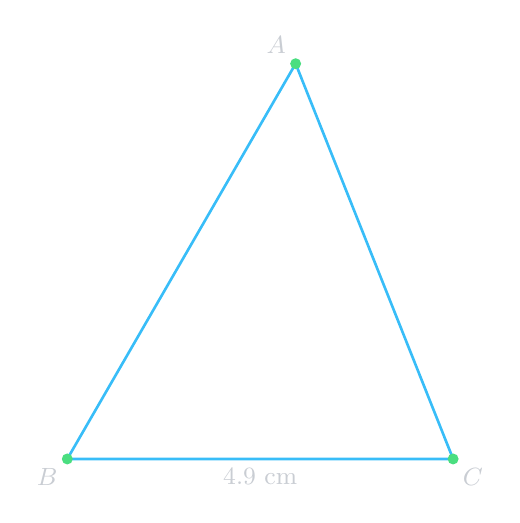
\begin{tikzpicture}[scale=1.0]
  \coordinate (B) at (0,0);
  \coordinate (C) at (4.9,0);
  \coordinate (A) at (2.9,5.02);

  \draw[tri] (A)--(B)--(C)--cycle;

  \node[pt] at (A) {}; \node[pt] at (B) {}; \node[pt] at (C) {};
  \node[labm,above left] at (A) {$A$};
  \node[labm,below left] at (B) {$B$};
  \node[labm,below right] at (C) {$C$};

  \node[labm,below] at ($(B)!0.5!(C)$) {$4.9$ cm};
\end{tikzpicture}
}

\StepPic{Step 5 (Draw bisectors of $\angle A$ and $\angle B$; they meet at $I$)}{
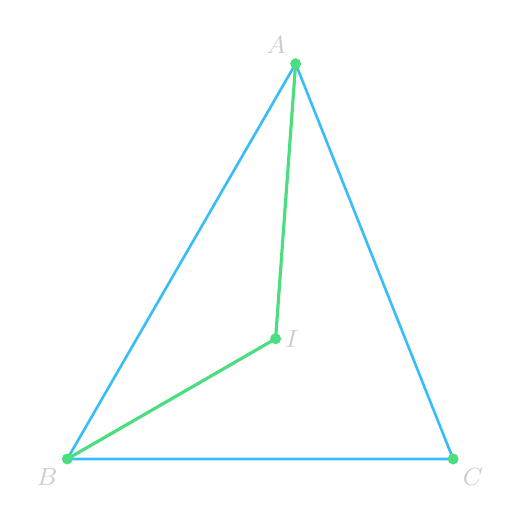
\begin{tikzpicture}[scale=1.0]
  \coordinate (B) at (0,0);
  \coordinate (C) at (4.9,0);
  \coordinate (A) at (2.9,5.02);

  % incenter (weights = side lengths approx)
  \coordinate (I) at (barycentric cs:A=4.9,B=5.41,C=5.8);

  \draw[tri] (A)--(B)--(C)--cycle;

  % bisectors shown (conceptual)
  \draw[special] (A)--(I);
  \draw[special] (B)--(I);

  \node[pt] at (A) {}; \node[pt] at (B) {}; \node[pt] at (C) {};
  \node[pt] at (I) {};
  \node[labm,above left] at (A) {$A$};
  \node[labm,below left] at (B) {$B$};
  \node[labm,below right] at (C) {$C$};
  \node[labm,right] at (I) {$I$};
\end{tikzpicture}
}

\StepPic{Step 6 (Draw bisector of $\angle C$; it also passes through $I$)}{
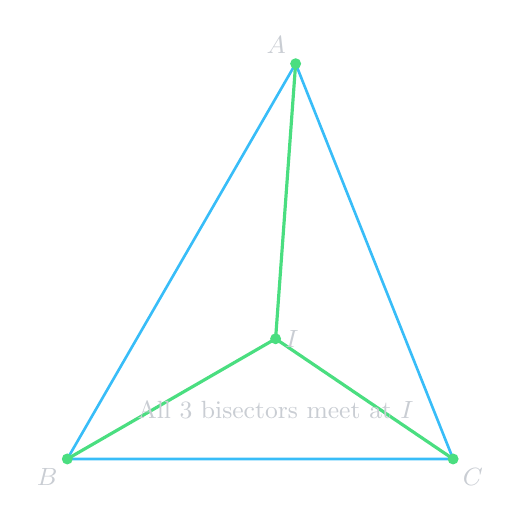
\begin{tikzpicture}[scale=1.0]
  \coordinate (B) at (0,0);
  \coordinate (C) at (4.9,0);
  \coordinate (A) at (2.9,5.02);
  \coordinate (I) at (barycentric cs:A=4.9,B=5.41,C=5.8);

  \draw[tri] (A)--(B)--(C)--cycle;
  \draw[special] (A)--(I);
  \draw[special] (B)--(I);
  \draw[special] (C)--(I);

  \node[pt] at (A) {}; \node[pt] at (B) {}; \node[pt] at (C) {};
  \node[pt] at (I) {};
  \node[labm,above left] at (A) {$A$};
  \node[labm,below left] at (B) {$B$};
  \node[labm,below right] at (C) {$C$};
  \node[labm,right] at (I) {$I$};

  \node[labm] at ($(I)+(0.0,-0.9)$) {All 3 bisectors meet at $I$};
\end{tikzpicture}
}

\textcolor{muted}{Reason (why this proves concurrency):} We constructed two angle bisectors and got their intersection $I$.  
Then the third bisector also passes through $I$ (incentre property), so the three bisectors are concurrent.
\end{QAPair}

% ============================================================
% Q1(b) - Angle bisectors concurrent
\begin{QAPair}{Question 1 (b)}
\textcolor{gold}{\bfseries Question:} Show that angle bisectors of $\triangle XYZ$ are concurrent when $XY=5.5$ cm, $\angle X=45^\circ$, $\angle Y=75^\circ$.

\tcblower
\textcolor{green}{\bfseries Construction + concurrency (step diagrams):}

\[
\begin{aligned}
\Step{1}\;& \text{Draw }XY=5.5\text{ cm.}\\
\Step{2}\;& \text{At }X,\ \text{construct }45^\circ\text{ and draw ray }XZ.\\
\Step{3}\;& \text{At }Y,\ \text{construct }75^\circ\text{ and draw ray }YZ.\\
\Step{4}\;& \text{Rays meet at }Z;\ \text{join to form }\triangle XYZ.\\
\Step{5}\;& \text{Draw bisectors of }\angle X \text{ and }\angle Y;\ \text{they meet at }I.\\
\Step{6}\;& \text{Draw bisector of }\angle Z;\ \text{it also passes through }I \Rightarrow \text{concurrent.}
\end{aligned}
\]

\StepPic{Step 1 (Draw base $XY=5.5$ cm)}{

\begin{tikzpicture}[scale=1.0]
  \coordinate (X) at (0,0);
  \coordinate (Y) at (5.5,0);
  \draw[tri] (X)--(Y);
  \node[pt] at (X) {}; \node[pt] at (Y) {};
  \node[labm,below left] at (X) {$X$};
  \node[labm,below right] at (Y) {$Y$};
  \node[labm,below] at ($(X)!0.5!(Y)$) {$5.5$ cm};
\end{tikzpicture}
}

\StepPic{Step 2 (At $X$ make $45^\circ$ and draw ray $XZ$)}{
\begin{tikzpicture}[scale=1.0]
  \coordinate (X) at (0,0);
  \coordinate (Y) at (5.5,0);
  \draw[tri] (X)--(Y);

  \draw[aux] (X)--+(45:5.3);
  \draw[aux] (X) ++(1.0,0) arc(0:45:1.0);
  \node[labm] at ($(X)+(0.95,0.35)$) {$45^\circ$};

  \node[pt] at (X) {}; \node[pt] at (Y) {};
  \node[labm,below left] at (X) {$X$};
  \node[labm,below right] at (Y) {$Y$};
\end{tikzpicture}
}

\StepPic{Step 3 (At $Y$ make $75^\circ$ and draw ray $YZ$)}{
\begin{tikzpicture}[scale=1.0]
  \coordinate (X) at (0,0);
  \coordinate (Y) at (5.5,0);
  \draw[tri] (X)--(Y);

  % interior angle at Y is 75 with YX (left), so ray direction is 180-75=105
  \draw[aux] (X)--+(45:5.3);
  \draw[aux] (Y)--+(105:5.5);

  \draw[aux] (X) ++(1.0,0) arc(0:45:1.0);
  \node[labm] at ($(X)+(0.95,0.35)$) {$45^\circ$};

  \draw[aux] (Y) ++(-1.0,0) arc(180:105:1.0);
  \node[labm] at ($(Y)+(-0.85,0.55)$) {$75^\circ$};

  \node[pt] at (X) {}; \node[pt] at (Y) {};
  \node[labm,below left] at (X) {$X$};
  \node[labm,below right] at (Y) {$Y$};
\end{tikzpicture}
}

\StepPic{Step 4 (Rays meet at $Z$; join sides)}{
\begin{tikzpicture}[scale=1.0]
  \coordinate (X) at (0,0);
  \coordinate (Y) at (5.5,0);

  \path[name path=rayX] (X) -- +(45:8);
  \path[name path=rayY] (Y) -- +(105:8);
  \path[name intersections={of=rayX and rayY, by=Z}];

  \draw[tri] (X)--(Y)--(Z)--cycle;

  % keep construction rays visible
  \draw[aux] (X)--+(45:5.8);
  \draw[aux] (Y)--+(105:5.8);

  \node[pt] at (X) {}; \node[pt] at (Y) {}; \node[pt] at (Z) {};
  \node[labm,below left] at (X) {$X$};
  \node[labm,below right] at (Y) {$Y$};
  \node[labm,above] at (Z) {$Z$};
\end{tikzpicture}
}

\StepPic{Step 5 (Draw bisectors of $\angle X$ and $\angle Y$; they meet at $I$)}{
\begin{tikzpicture}[scale=1.0]
  \coordinate (X) at (0,0);
  \coordinate (Y) at (5.5,0);
  \path[name path=rayX] (X) -- +(45:8);
  \path[name path=rayY] (Y) -- +(105:8);
  \path[name intersections={of=rayX and rayY, by=Z}];

  % choose an incenter-like point (conceptual) using barycentric weights
  \coordinate (I) at (barycentric cs:X=4.9,Y=5.0,Z=5.4);

  \draw[tri] (X)--(Y)--(Z)--cycle;
  \draw[special] (X)--(I);
  \draw[special] (Y)--(I);

  \node[pt] at (X) {}; \node[pt] at (Y) {}; \node[pt] at (Z) {};
  \node[pt] at (I) {};
  \node[labm,below left] at (X) {$X$};
  \node[labm,below right] at (Y) {$Y$};
  \node[labm,above] at (Z) {$Z$};
  \node[labm,right] at (I) {$I$};
\end{tikzpicture}
}

\StepPic{Step 6 (Draw bisector of $\angle Z$; it also passes through $I$)}{
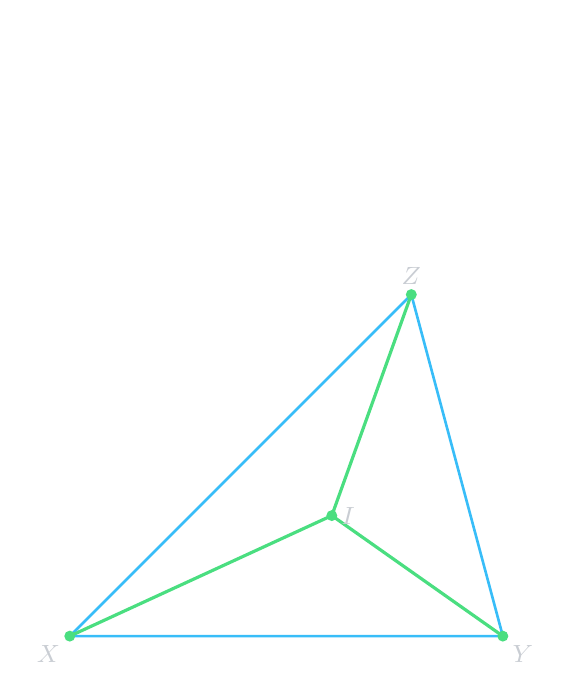
\begin{tikzpicture}[scale=1.0]
  \coordinate (X) at (0,0);
  \coordinate (Y) at (5.5,0);
  \path[name path=rayX] (X) -- +(45:8);
  \path[name path=rayY] (Y) -- +(105:8);
  \path[name intersections={of=rayX and rayY, by=Z}];

  \coordinate (I) at (barycentric cs:X=4.9,Y=5.0,Z=5.4);

  \draw[tri] (X)--(Y)--(Z)--cycle;
  \draw[special] (X)--(I);
  \draw[special] (Y)--(I);
  \draw[special] (Z)--(I);

  \node[pt] at (X) {}; \node[pt] at (Y) {}; \node[pt] at (Z) {};
  \node[pt] at (I) {};
  \node[labm,below left] at (X) {$X$};
  \node[labm,below right] at (Y) {$Y$};
  \node[labm,above] at (Z) {$Z$};
  \node[labm,right] at (I) {$I$};
\end{tikzpicture}
}
\end{QAPair}

% ============================================================
% Q2(a) - Altitudes concurrent
\begin{QAPair}{Question 2 (a)}
\textcolor{gold}{\bfseries Question:} Show that altitudes of $\triangle ABC$ are concurrent when $AB=4$ cm, $BC=5$ cm, $AC=6$ cm.

\tcblower
\textcolor{green}{\bfseries Construction + orthocentre (step diagrams):}

\[
\begin{aligned}
\Step{1}\;& \text{Draw }AC=6\text{ cm.}\\
\Step{2}\;& \text{With centre }A\text{ radius }4\text{ cm and centre }C\text{ radius }5\text{ cm, draw arcs to meet at }B.\\
\Step{3}\;& \text{Join }AB\text{ and }BC\text{ to form }\triangle ABC.\\
\Step{4}\;& \text{Draw altitude }AD\perp BC.\\
\Step{5}\;& \text{Draw altitude }BE\perp AC;\ \text{let }AD\cap BE=H.\\
\Step{6}\;& \text{Draw altitude }CF\perp AB;\ \text{it passes through }H \Rightarrow \text{concurrent at }H.
\end{aligned}
\]

\StepPic{Step 1 (Draw base $AC=6$ cm)}{

\begin{tikzpicture}[scale=1.0]
  \coordinate (A) at (0,0);
  \coordinate (C) at (6,0);
  \draw[tri] (A)--(C);
  \node[pt] at (A) {}; \node[pt] at (C) {};
  \node[labm,below left] at (A) {$A$};
  \node[labm,below right] at (C) {$C$};
  \node[labm,below] at ($(A)!0.5!(C)$) {$6$ cm};
\end{tikzpicture}
}

\StepPic{Step 2 (Draw arcs: centre $A$, radius 4; centre $C$, radius 5)}{
\begin{tikzpicture}[scale=1.0]
  \coordinate (A) at (0,0);
  \coordinate (C) at (6,0);
  \draw[tri] (A)--(C);

  \draw[aux] (A) circle (4);
  \draw[aux] (C) circle (5);

  \node[pt] at (A) {}; \node[pt] at (C) {};
  \node[labm,below left] at (A) {$A$};
  \node[labm,below right] at (C) {$C$};
  \node[labm] at ($(A)+(2.6,2.9)$) {$r=4$};
  \node[labm] at ($(C)+(-3.0,3.5)$) {$r=5$};
\end{tikzpicture}
}

\StepPic{Step 3 (Arcs meet at $B$; join to form $\triangle ABC$)}{
\begin{tikzpicture}[scale=1.0]
  \coordinate (A) at (0,0);
  \coordinate (C) at (6,0);
  % pick B roughly consistent with 4 and 5 (schematic)
  \coordinate (B) at (2.0,3.46);

  \draw[aux] (A) circle (4);
  \draw[aux] (C) circle (5);

  \draw[tri] (A)--(B)--(C)--cycle;

  \node[pt] at (A) {}; \node[pt] at (B) {}; \node[pt] at (C) {};
  \node[labm,below left] at (A) {$A$};
  \node[labm,above] at (B) {$B$};
  \node[labm,below right] at (C) {$C$};

  \node[labm] at ($(A)!0.5!(B)$) {$AB=4$};
  \node[labm] at ($(B)!0.5!(C)$) {$BC=5$};
  \node[labm,below] at ($(A)!0.5!(C)$) {$AC=6$};
\end{tikzpicture}
}

\StepPic{Step 4 (Draw altitude $AD\perp BC$)}{
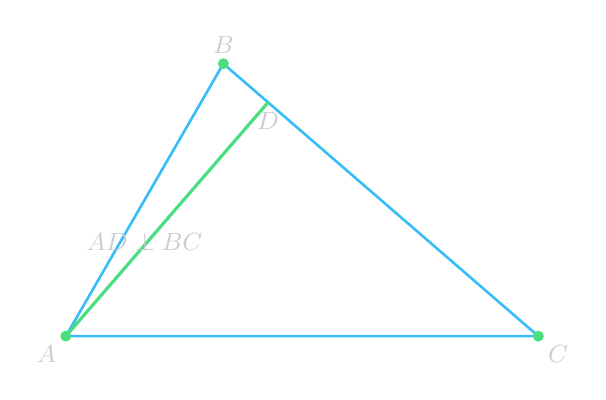
\begin{tikzpicture}[scale=1.0]
  \coordinate (A) at (0,0);
  \coordinate (C) at (6,0);
  \coordinate (B) at (2.0,3.46);

  \coordinate (D) at ($(B)!(A)!(C)$); % foot from A to BC? (schematic)
  % Better: foot from A to BC:
  \coordinate (D) at ($(B)!(A)!(C)$);

  \draw[tri] (A)--(B)--(C)--cycle;

  % altitude from A to BC (use projection of A onto BC)
  \coordinate (D) at ($(B)!(A)!(C)$); % OK for a schematic line to BC direction
  \draw[special] (A)--(D);

  \node[pt] at (A) {}; \node[pt] at (B) {}; \node[pt] at (C) {};
  \node[labm,below left] at (A) {$A$};
  \node[labm,above] at (B) {$B$};
  \node[labm,below right] at (C) {$C$};
  \node[labm,below] at (D) {$D$};

  \node[labm] at ($(A)+(1.0,1.2)$) {$AD\perp BC$};
\end{tikzpicture}
}

\StepPic{Step 5 (Draw altitude $BE\perp AC$; intersection is $H$)}{
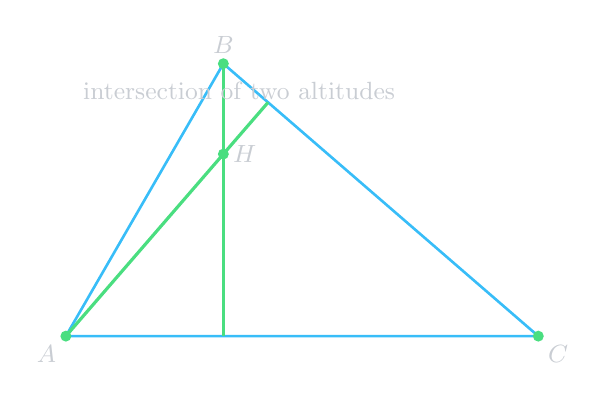
\begin{tikzpicture}[scale=1.0]
  \coordinate (A) at (0,0);
  \coordinate (C) at (6,0);
  \coordinate (B) at (2.0,3.46);

  \coordinate (E) at ($(A)!(B)!(C)$); % foot from B to AC
  \coordinate (D) at ($(B)!(A)!(C)$);

  % intersection H of altitudes (schematic)
  \path[name path=altA] (A)--(D);
  \path[name path=altB] (B)--(E);
  \path[name intersections={of=altA and altB, by=H}];

  \draw[tri] (A)--(B)--(C)--cycle;
  \draw[special] (A)--(D);
  \draw[special] (B)--(E);

  \node[pt] at (A) {}; \node[pt] at (B) {}; \node[pt] at (C) {};
  \node[pt] at (H) {};
  \node[labm,below left] at (A) {$A$};
  \node[labm,above] at (B) {$B$};
  \node[labm,below right] at (C) {$C$};
  \node[labm,right] at (H) {$H$};

  \node[labm] at ($(H)+(0.2,0.8)$) {intersection of two altitudes};
\end{tikzpicture}
}

\StepPic{Step 6 (Draw altitude $CF\perp AB$; it also passes through $H$)}{
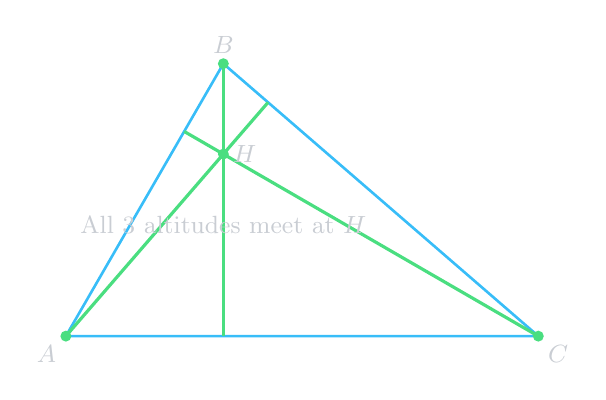
\begin{tikzpicture}[scale=1.0]
  \coordinate (A) at (0,0);
  \coordinate (C) at (6,0);
  \coordinate (B) at (2.0,3.46);

  \coordinate (E) at ($(A)!(B)!(C)$);
  \coordinate (D) at ($(B)!(A)!(C)$);
  \coordinate (F) at ($(A)!(C)!(B)$); % foot from C to AB (schematic)

  \path[name path=altA] (A)--(D);
  \path[name path=altB] (B)--(E);
  \path[name intersections={of=altA and altB, by=H}];

  \draw[tri] (A)--(B)--(C)--cycle;
  \draw[special] (A)--(D);
  \draw[special] (B)--(E);
  \draw[special] (C)--(F);

  \node[pt] at (A) {}; \node[pt] at (B) {}; \node[pt] at (C) {};
  \node[pt] at (H) {};
  \node[labm,below left] at (A) {$A$};
  \node[labm,above] at (B) {$B$};
  \node[labm,below right] at (C) {$C$};
  \node[labm,right] at (H) {$H$};

  \node[labm] at ($(H)+(0.0,-0.9)$) {All 3 altitudes meet at $H$};
\end{tikzpicture}
}
\end{QAPair}

% ============================================================
% Q2(b) - Altitudes in right triangle
\begin{QAPair}{Question 2 (b)}
\textcolor{gold}{\bfseries Question:} Show that altitudes of $\triangle PQR$ are concurrent when $PQ=4.6$ cm, $QR=6.5$ cm, $\angle P=90^\circ$.

\tcblower
\textcolor{green}{\bfseries Construction + orthocentre (step diagrams):}

\[
\begin{aligned}
\Step{1}\;& \text{At }P,\ \text{construct a right angle (two perpendicular rays).}\\
\Step{2}\;& \text{On one ray, mark }PQ=4.6\text{ cm.}\\
\Step{3}\;& \text{With centre }Q\text{ radius }6.5\text{ cm, cut the other ray at }R.\\
\Step{4}\;& \text{Join }QR\text{ and }PR\text{ to form }\triangle PQR.\\
\Step{5}\;& \text{In a right triangle, }PQ \text{ and }PR\text{ are themselves altitudes.}\\
\Step{6}\;& \Rightarrow \text{Altitudes meet at }P\ (\text{orthocentre}).
\end{aligned}
\]

\StepPic{Step 1 (Make $\angle P=90^\circ$)}{
\begin{tikzpicture}[scale=1.0]
  \coordinate (P) at (0,0);
  \draw[aux] (P)--+(5.0,0);
  \draw[aux] (P)--+(0,3.8);
  \RightMarkAt{P}
  \node[pt] at (P) {};
  \node[labm,below left] at (P) {$P$};
\end{tikzpicture}
}

\StepPic{Step 2 (Mark $PQ=4.6$ cm)}{
\begin{tikzpicture}[scale=1.0]
  \coordinate (P) at (0,0);
  \coordinate (Q) at (4.6,0);
  \draw[aux] (P)--+(5.2,0);
  \draw[aux] (P)--+(0,3.8);
  \RightMarkAt{P}

  \draw[tri] (P)--(Q);
  \node[pt] at (P) {}; \node[pt] at (Q) {};
  \node[labm,below left] at (P) {$P$};
  \node[labm,below right] at (Q) {$Q$};
  \node[labm,below] at ($(P)!0.5!(Q)$) {$4.6$ cm};
\end{tikzpicture}
}

\StepPic{Step 3 (Arc with centre $Q$, radius $6.5$ cm meets other ray at $R$)}{
\begin{tikzpicture}[scale=0.9]
  \coordinate (P) at (0,0);
  \coordinate (Q) at (4.6,0);

  \draw[aux] (P)--+(6.0,0);
  \draw[aux] (P)--+(0,5.0);
  \RightMarkAt{P}

  \draw[tri] (P)--(Q);
  \draw[aux] (Q) circle (6.5);

  % choose a point on the vertical ray as "R" (schematic)
  \coordinate (R) at (0,4.6);

  \node[pt] at (P) {}; \node[pt] at (Q) {}; \node[pt] at (R) {};
  \node[labm,below left] at (P) {$P$};
  \node[labm,below right] at (Q) {$Q$};
  \node[labm,left] at (R) {$R$};

  \node[labm] at ($(Q)+(2.6,2.8)$) {$r=6.5$};
\end{tikzpicture}
}

\StepPic{Step 4 (Join to form $\triangle PQR$)}{
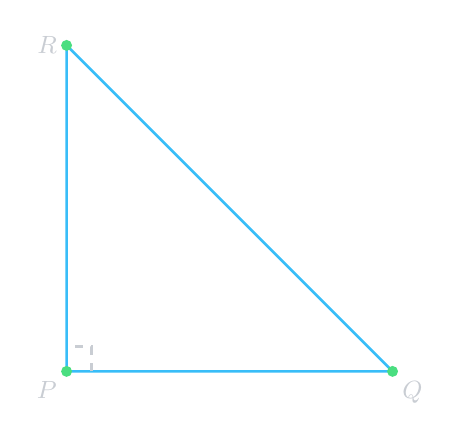
\begin{tikzpicture}[scale=0.9]
  \coordinate (P) at (0,0);
  \coordinate (Q) at (4.6,0);
  \coordinate (R) at (0,4.6);

  \draw[tri] (P)--(Q)--(R)--cycle;
  \RightMarkAt{P}

  \node[pt] at (P) {}; \node[pt] at (Q) {}; \node[pt] at (R) {};
  \node[labm,below left] at (P) {$P$};
  \node[labm,below right] at (Q) {$Q$};
  \node[labm,left] at (R) {$R$};
\end{tikzpicture}
}

\StepPic{Step 5 (Show altitudes: the legs $PQ$ and $PR$)}{
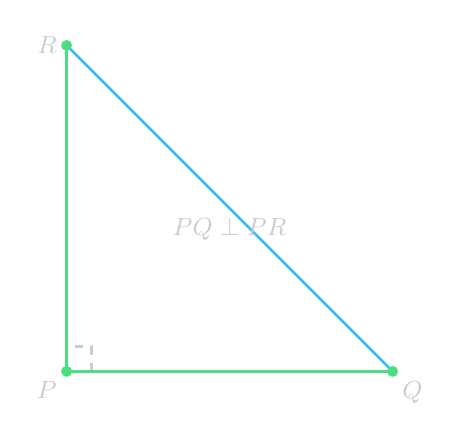
\begin{tikzpicture}[scale=0.9]
  \coordinate (P) at (0,0);
  \coordinate (Q) at (4.6,0);
  \coordinate (R) at (0,4.6);

  \draw[tri] (P)--(Q)--(R)--cycle;
  \RightMarkAt{P}

  \draw[special] (P)--(Q);
  \draw[special] (P)--(R);

  \node[pt] at (P) {}; \node[pt] at (Q) {}; \node[pt] at (R) {};
  \node[labm,below left] at (P) {$P$};
  \node[labm,below right] at (Q) {$Q$};
  \node[labm,left] at (R) {$R$};

  \node[labm] at ($(P)+(2.3,2.0)$) {$PQ\perp PR$};
\end{tikzpicture}
}

\StepPic{Step 6 (Altitudes meet at $P$: orthocentre)}{
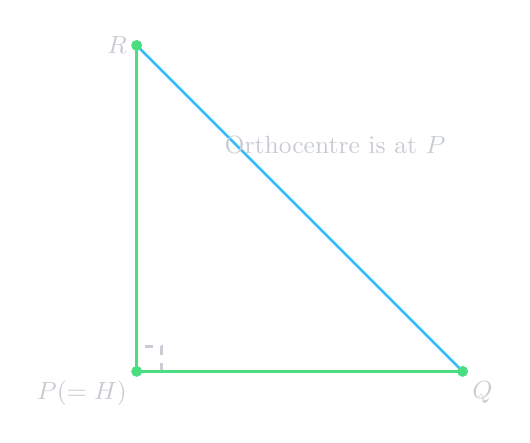
\begin{tikzpicture}[scale=0.9]
  \coordinate (P) at (0,0);
  \coordinate (Q) at (4.6,0);
  \coordinate (R) at (0,4.6);

  \draw[tri] (P)--(Q)--(R)--cycle;
  \RightMarkAt{P}

  \draw[special] (P)--(Q);
  \draw[special] (P)--(R);

  \node[pt] at (P) {}; \node[pt] at (Q) {}; \node[pt] at (R) {};
  \node[labm,below left] at (P) {$P(=H)$};
  \node[labm,below right] at (Q) {$Q$};
  \node[labm,left] at (R) {$R$};

  \node[labm] at ($(P)+(2.8,3.2)$) {Orthocentre is at $P$};
\end{tikzpicture}
}
\end{QAPair}

% ============================================================
% Q2(c) - Altitudes concurrent in obtuse triangle
\begin{QAPair}{Question 2 (c)}
\textcolor{gold}{\bfseries Question:} Show that altitudes of $\triangle LMN$ are concurrent when $LM=4.2$ cm, $MN=4$ cm, $\angle M=105^\circ$.

\tcblower
\textcolor{green}{\bfseries Construction + orthocentre (step diagrams):}

\[
\begin{aligned}
\Step{1}\;& \text{At }M,\ \text{construct }105^\circ\text{ (two rays).}\\
\Step{2}\;& \text{On one arm mark }MN=4\text{ cm; on the other mark }ML=4.2\text{ cm.}\\
\Step{3}\;& \text{Join }L\text{ to }N\text{ to form }\triangle LMN.\\
\Step{4}\;& \text{Draw altitude from }L\text{ to }MN.\\
\Step{5}\;& \text{Draw altitude from }N\text{ to }LM;\ \text{they meet at }H.\\
\Step{6}\;& \text{The third altitude from }M\text{ also passes through }H \Rightarrow \text{concurrent.}
\end{aligned}
\]

\StepPic{Step 1 (At $M$ make $105^\circ$)}{
\begin{tikzpicture}[scale=1.0]
  \coordinate (M) at (0,0);
  \draw[aux] (M)--+(5.5,0);
  \draw[aux] (M)--+(105:5.2);
  \draw[aux] (M) ++(1.0,0) arc(0:105:1.0);
  \node[labm] at ($(M)+(0.55,1.05)$) {$105^\circ$};
  \node[pt] at (M) {};
  \node[labm,below] at (M) {$M$};
\end{tikzpicture}
}

\StepPic{Step 2 (Mark $MN=4$ and $ML=4.2$)}{
\begin{tikzpicture}[scale=0.95]
  \coordinate (M) at (0,0);
  \coordinate (N) at (4,0);
  \coordinate (L) at ($(M)+(105:4.2)$);

  \draw[aux] (M)--+(5.5,0);
  \draw[aux] (M)--+(105:5.2);
  \draw[tri] (M)--(N);
  \draw[tri] (M)--(L);

  \node[pt] at (M) {}; \node[pt] at (N) {}; \node[pt] at (L) {};
  \node[labm,below] at (M) {$M$};
  \node[labm,below right] at (N) {$N$};
  \node[labm,above left] at (L) {$L$};

  \node[labm,below] at ($(M)!0.5!(N)$) {$4$ cm};
  \node[labm,left] at ($(M)!0.5!(L)$) {$4.2$ cm};
\end{tikzpicture}
}

\StepPic{Step 3 (Join $L$ to $N$ to complete the triangle)}{
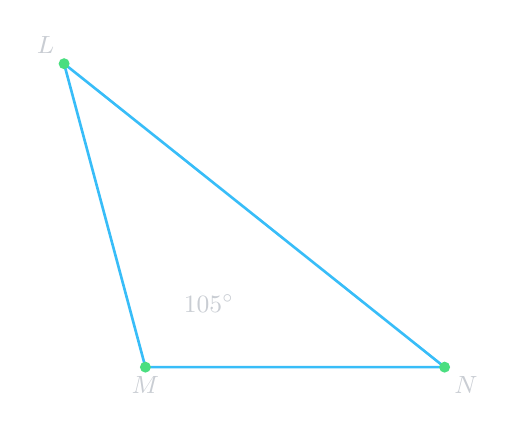
\begin{tikzpicture}[scale=0.95]
  \coordinate (M) at (0,0);
  \coordinate (N) at (4,0);
  \coordinate (L) at ($(M)+(105:4.2)$);

  \draw[tri] (L)--(M)--(N)--cycle;

  \node[pt] at (M) {}; \node[pt] at (N) {}; \node[pt] at (L) {};
  \node[labm,below] at (M) {$M$};
  \node[labm,below right] at (N) {$N$};
  \node[labm,above left] at (L) {$L$};

  \node[labm] at ($(M)+(0.85,0.85)$) {$105^\circ$};
\end{tikzpicture}
}

\StepPic{Step 4 (Draw altitude from $L$ to $MN$)}{
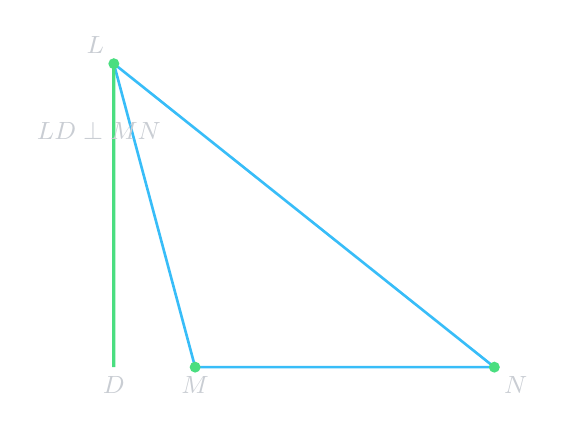
\begin{tikzpicture}[scale=0.95]
  \coordinate (M) at (0,0);
  \coordinate (N) at (4,0);
  \coordinate (L) at ($(M)+(105:4.2)$);
  \coordinate (D) at ($(M)!(L)!(N)$); % projection of L onto MN

  \draw[tri] (L)--(M)--(N)--cycle;
  \draw[special] (L)--(D);

  \node[pt] at (L) {}; \node[pt] at (M) {}; \node[pt] at (N) {};
  \node[labm,above left] at (L) {$L$};
  \node[labm,below] at (M) {$M$};
  \node[labm,below right] at (N) {$N$};
  \node[labm,below] at (D) {$D$};

  \node[labm] at ($(L)+(-0.2,-0.9)$) {$LD\perp MN$};
\end{tikzpicture}
}

\StepPic{Step 5 (Draw altitude from $N$ to $LM$; meet at $H$)}{
\begin{tikzpicture}[scale=0.95]
  \coordinate (M) at (0,0);
  \coordinate (N) at (4,0);
  \coordinate (L) at ($(M)+(105:4.2)$);

  \coordinate (D) at ($(M)!(L)!(N)$);
  \coordinate (E) at ($(L)!(N)!(M)$); % projection of N onto LM

  \path[name path=altL] (L)--(D);
  \path[name path=altN] (N)--(E);
  \path[name intersections={of=altL and altN, by=H}];

  \draw[tri] (L)--(M)--(N)--cycle;
  \draw[special] (L)--(D);
  \draw[special] (N)--(E);

  \node[pt] at (L) {}; \node[pt] at (M) {}; \node[pt] at (N) {};
  \node[pt] at (H) {};
  \node[labm,above left] at (L) {$L$};
  \node[labm,below] at (M) {$M$};
  \node[labm,below right] at (N) {$N$};
  \node[labm,right] at (H) {$H$};

  \node[labm] at ($(H)+(0.1,0.8)$) {intersection of two altitudes};
\end{tikzpicture}
}

\StepPic{Step 6 (Third altitude from $M$ also passes through $H$)}{
\begin{tikzpicture}[scale=0.95]
  \coordinate (M) at (0,0);
  \coordinate (N) at (4,0);
  \coordinate (L) at ($(M)+(105:4.2)$);

  \coordinate (D) at ($(M)!(L)!(N)$);
  \coordinate (E) at ($(L)!(N)!(M)$);
  \coordinate (F) at ($(N)!(M)!(L)$); % projection of M onto LN (schematic)

  \path[name path=altL] (L)--(D);
  \path[name path=altN] (N)--(E);
  \path[name intersections={of=altL and altN, by=H}];

  \draw[tri] (L)--(M)--(N)--cycle;
  \draw[special] (L)--(D);
  \draw[special] (N)--(E);
  \draw[special] (M)--(F);

  \node[pt] at (L) {}; \node[pt] at (M) {}; \node[pt] at (N) {};
  \node[pt] at (H) {};
  \node[labm,above left] at (L) {$L$};
  \node[labm,below] at (M) {$M$};
  \node[labm,below right] at (N) {$N$};
  \node[labm,right] at (H) {$H$};

  \node[labm] at ($(H)+(0.0,-1.0)$) {All 3 altitudes meet at $H$ (outside if obtuse)};
\end{tikzpicture}
}
\end{QAPair}

% ============================================================
% Q3(a) - Perpendicular bisectors concurrent
\begin{QAPair}{Question 3 (a)}
\textcolor{gold}{\bfseries Question:} Show that perpendicular bisectors of $\triangle XYZ$ are concurrent when $XY=4.5$ cm, $YZ=5$ cm, $ZX=4.8$ cm.

\tcblower
\textcolor{green}{\bfseries Construction + circumcentre (step diagrams):}

\[
\begin{aligned}
\Step{1}\;& \text{Draw }XY=4.5\text{ cm.}\\
\Step{2}\;& \text{With centre }X\text{ radius }4.8\text{ cm and centre }Y\text{ radius }5\text{ cm, draw arcs to locate }Z.\\
\Step{3}\;& \text{Join }XZ\text{ and }YZ\text{ to form }\triangle XYZ.\\
\Step{4}\;& \text{Draw perpendicular bisector of }XY.\\
\Step{5}\;& \text{Draw perpendicular bisector of }YZ;\ \text{they meet at }O.\\
\Step{6}\;& \text{Draw perpendicular bisector of }ZX;\ \text{it also passes through }O \Rightarrow \text{concurrent at }O.
\end{aligned}
\]

\StepPic{Step 1 (Draw base $XY=4.5$ cm)}{

\begin{tikzpicture}[scale=1.0]
  \coordinate (X) at (0,0);
  \coordinate (Y) at (4.5,0);
  \draw[tri] (X)--(Y);
  \node[pt] at (X) {}; \node[pt] at (Y) {};
  \node[labm,below left] at (X) {$X$};
  \node[labm,below right] at (Y) {$Y$};
  \node[labm,below] at ($(X)!0.5!(Y)$) {$4.5$ cm};
\end{tikzpicture}
}

\StepPic{Step 2 (Draw arcs to locate $Z$)}{
\begin{tikzpicture}[scale=1.0]
  \coordinate (X) at (0,0);
  \coordinate (Y) at (4.5,0);
  \draw[tri] (X)--(Y);

  \draw[aux] (X) circle (4.8);
  \draw[aux] (Y) circle (5.0);

  \node[pt] at (X) {}; \node[pt] at (Y) {};
  \node[labm,below left] at (X) {$X$};
  \node[labm,below right] at (Y) {$Y$};
  \node[labm] at ($(X)+(2.7,3.1)$) {$r=4.8$};
  \node[labm] at ($(Y)+(-3.0,3.4)$) {$r=5$};
\end{tikzpicture}
}

\StepPic{Step 3 (Arcs meet at $Z$; join to form triangle)}{
\begin{tikzpicture}[scale=1.0]
  \coordinate (X) at (0,0);
  \coordinate (Y) at (4.5,0);
  \coordinate (Z) at (1.8,3.7); % schematic meeting point

  \draw[aux] (X) circle (4.8);
  \draw[aux] (Y) circle (5.0);

  \draw[tri] (X)--(Y)--(Z)--cycle;

  \node[pt] at (X) {}; \node[pt] at (Y) {}; \node[pt] at (Z) {};
  \node[labm,below left] at (X) {$X$};
  \node[labm,below right] at (Y) {$Y$};
  \node[labm,above] at (Z) {$Z$};
\end{tikzpicture}
}

\StepPic{Step 4 (Draw perpendicular bisector of $XY$)}{
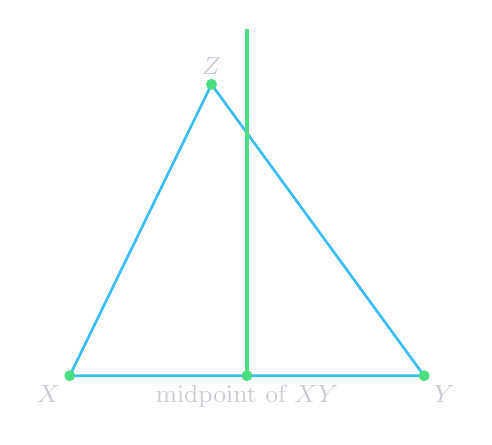
\begin{tikzpicture}[scale=1.0]
  \coordinate (X) at (0,0);
  \coordinate (Y) at (4.5,0);
  \coordinate (Z) at (1.8,3.7);
  \coordinate (M) at ($(X)!0.5!(Y)$);

  \draw[tri] (X)--(Y)--(Z)--cycle;
  \draw[special] (M)--+(0,4.4); % perp bisector of XY (schematic vertical)
  \node[pt] at (M) {};
  \node[labm,below] at (M) {midpoint of $XY$};

  \node[pt] at (X) {}; \node[pt] at (Y) {}; \node[pt] at (Z) {};
  \node[labm,below left] at (X) {$X$};
  \node[labm,below right] at (Y) {$Y$};
  \node[labm,above] at (Z) {$Z$};
\end{tikzpicture}
}

\StepPic{Step 5 (Draw perpendicular bisector of $YZ$; meet at $O$)}{
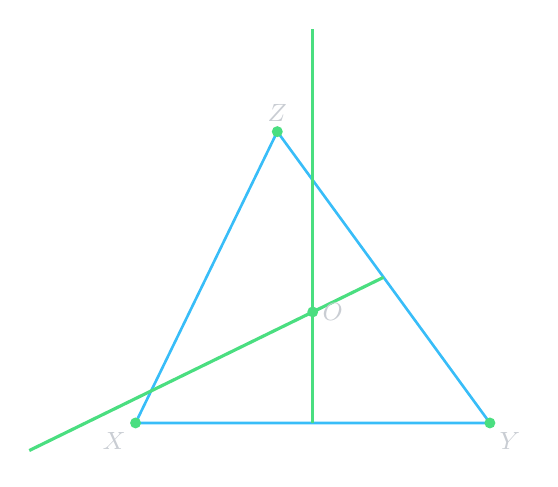
\begin{tikzpicture}[scale=1.0]
  \coordinate (X) at (0,0);
  \coordinate (Y) at (4.5,0);
  \coordinate (Z) at (1.8,3.7);

  \coordinate (Mxy) at ($(X)!0.5!(Y)$);
  \coordinate (Myz) at ($(Y)!0.5!(Z)$);

  % two bisectors (schematic)
  \path[name path=bxy] (Mxy) -- +(0,5);
  \path[name path=byz] (Myz) -- +(-4.5,-2.2);
  \path[name intersections={of=bxy and byz, by=O}];

  \draw[tri] (X)--(Y)--(Z)--cycle;
  \draw[special] (Mxy)--+(0,5);
  \draw[special] (Myz)--+(-4.5,-2.2);

  \node[pt] at (O) {};
  \node[labm,right] at (O) {$O$};

  \node[pt] at (X) {}; \node[pt] at (Y) {}; \node[pt] at (Z) {};
  \node[labm,below left] at (X) {$X$};
  \node[labm,below right] at (Y) {$Y$};
  \node[labm,above] at (Z) {$Z$};
\end{tikzpicture}
}

\StepPic{Step 6 (Third bisector of $ZX$ also passes through $O$)}{
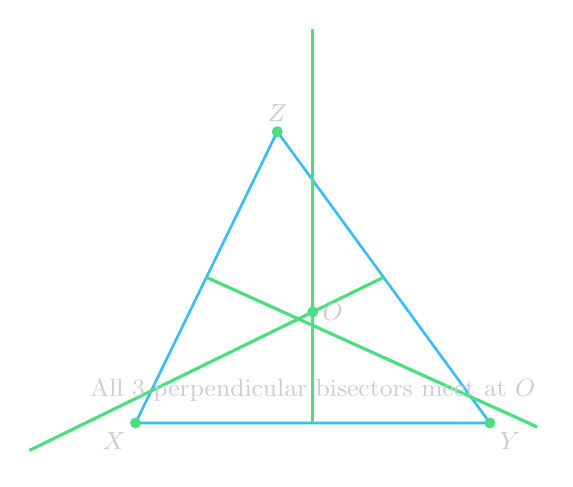
\begin{tikzpicture}[scale=1.0]
  \coordinate (X) at (0,0);
  \coordinate (Y) at (4.5,0);
  \coordinate (Z) at (1.8,3.7);

  \coordinate (Mxy) at ($(X)!0.5!(Y)$);
  \coordinate (Myz) at ($(Y)!0.5!(Z)$);
  \coordinate (Mzx) at ($(Z)!0.5!(X)$);

  \path[name path=bxy] (Mxy) -- +(0,5);
  \path[name path=byz] (Myz) -- +(-4.5,-2.2);
  \path[name intersections={of=bxy and byz, by=O}];

  \draw[tri] (X)--(Y)--(Z)--cycle;
  \draw[special] (Mxy)--+(0,5);
  \draw[special] (Myz)--+(-4.5,-2.2);
  \draw[special] (Mzx)--+(4.2,-1.9); % third bisector (schematic)

  \node[pt] at (O) {};
  \node[labm,right] at (O) {$O$};
  \node[labm] at ($(O)+(0.0,-1.0)$) {All 3 perpendicular bisectors meet at $O$};

  \node[pt] at (X) {}; \node[pt] at (Y) {}; \node[pt] at (Z) {};
  \node[labm,below left] at (X) {$X$};
  \node[labm,below right] at (Y) {$Y$};
  \node[labm,above] at (Z) {$Z$};
\end{tikzpicture}
}
\end{QAPair}

% ============================================================
% Q3(b) - Perpendicular bisectors in right triangle
\begin{QAPair}{Question 3 (b)}
\textcolor{gold}{\bfseries Question:} Show that perpendicular bisectors of $\triangle PQR$ are concurrent when $PQ=4$ cm, $QR=5.8$ cm, $\angle Q=90^\circ$.

\tcblower
\textcolor{green}{\bfseries Construction + circumcentre (step diagrams):}

\[
\begin{aligned}
\Step{1}\;& \text{At }Q,\ \text{construct a right angle.}\\
\Step{2}\;& \text{Mark }QP=4\text{ cm on one arm and }QR=5.8\text{ cm on the other arm.}\\
\Step{3}\;& \text{Join }PR\text{ to form }\triangle PQR.\\
\Step{4}\;& \text{Find midpoint }M\text{ of hypotenuse }PR.\\
\Step{5}\;& \text{Draw perpendicular bisector of }PQ\text{ and of }QR;\ \text{they meet at }M.\\
\Step{6}\;& \Rightarrow \text{All perpendicular bisectors are concurrent at }M\ (\text{midpoint of hypotenuse}).
\end{aligned}
\]

\StepPic{Step 1 (Right angle at $Q$)}{
\begin{tikzpicture}[scale=1.0]
  \coordinate (Q) at (0,0);
  \draw[aux] (Q)--+(5.2,0);
  \draw[aux] (Q)--+(0,4.2);
  \RightMarkAt{Q}
  \node[pt] at (Q) {};
  \node[labm,below left] at (Q) {$Q$};
\end{tikzpicture}
}

\StepPic{Step 2 (Mark $QP=4$ cm and $QR=5.8$ cm)}{
\begin{tikzpicture}[scale=0.9]
  \coordinate (Q) at (0,0);
  \coordinate (P) at (4,0);
  \coordinate (R) at (0,5.8);

  \draw[tri] (Q)--(P);
  \draw[tri] (Q)--(R);
  \RightMarkAt{Q}

  \node[pt] at (Q) {}; \node[pt] at (P) {}; \node[pt] at (R) {};
  \node[labm,below left] at (Q) {$Q$};
  \node[labm,below right] at (P) {$P$};
  \node[labm,left] at (R) {$R$};

  \node[labm,below] at ($(Q)!0.5!(P)$) {$4$ cm};
  \node[labm,left] at ($(Q)!0.5!(R)$) {$5.8$ cm};
\end{tikzpicture}
}

\StepPic{Step 3 (Join $PR$ to form $\triangle PQR$)}{
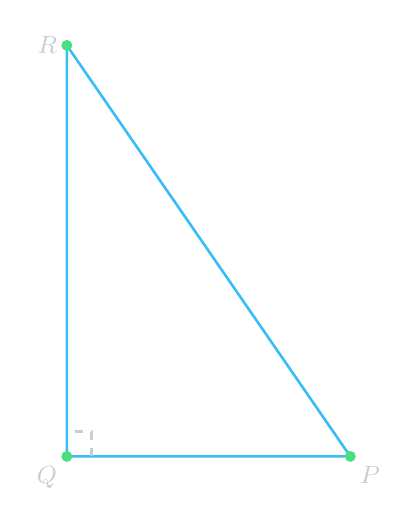
\begin{tikzpicture}[scale=0.9]
  \coordinate (Q) at (0,0);
  \coordinate (P) at (4,0);
  \coordinate (R) at (0,5.8);

  \draw[tri] (P)--(Q)--(R)--cycle;
  \RightMarkAt{Q}

  \node[pt] at (Q) {}; \node[pt] at (P) {}; \node[pt] at (R) {};
  \node[labm,below left] at (Q) {$Q$};
  \node[labm,below right] at (P) {$P$};
  \node[labm,left] at (R) {$R$};
\end{tikzpicture}
}

\StepPic{Step 4 (Find midpoint $M$ of hypotenuse $PR$)}{
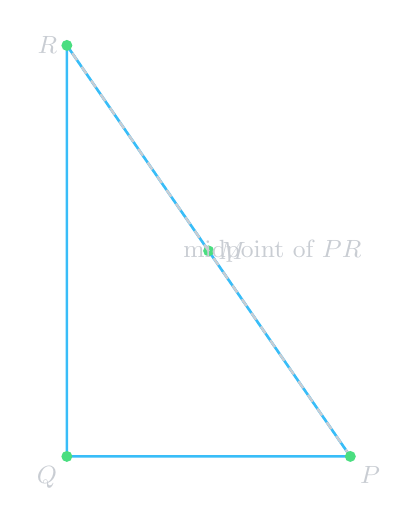
\begin{tikzpicture}[scale=0.9]
  \coordinate (Q) at (0,0);
  \coordinate (P) at (4,0);
  \coordinate (R) at (0,5.8);
  \coordinate (M) at ($(P)!0.5!(R)$);

  \draw[tri] (P)--(Q)--(R)--cycle;
  \node[pt] at (M) {};
  \node[labm,right] at (M) {$M$};
  \draw[aux] (P)--(R);
  \node[labm] at ($(P)!0.5!(R)+(0.9,0.0)$) {midpoint of $PR$};

  \node[pt] at (Q) {}; \node[pt] at (P) {}; \node[pt] at (R) {};
  \node[labm,below left] at (Q) {$Q$};
  \node[labm,below right] at (P) {$P$};
  \node[labm,left] at (R) {$R$};
\end{tikzpicture}
}

\StepPic{Step 5 (Perpendicular bisectors of $PQ$ and $QR$ meet at $M$)}{
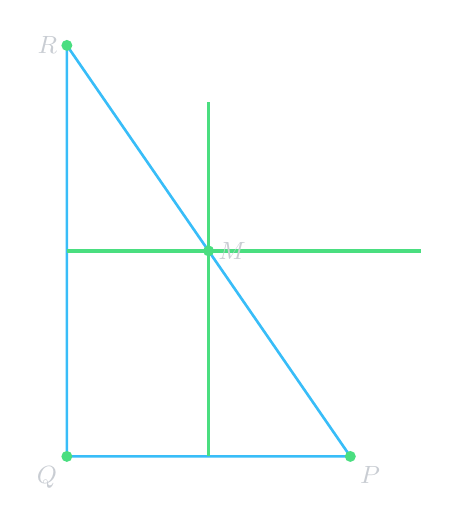
\begin{tikzpicture}[scale=0.9]
  \coordinate (Q) at (0,0);
  \coordinate (P) at (4,0);
  \coordinate (R) at (0,5.8);
  \coordinate (M) at ($(P)!0.5!(R)$);

  \coordinate (Mpq) at ($(P)!0.5!(Q)$);
  \coordinate (Mqr) at ($(Q)!0.5!(R)$);

  \draw[tri] (P)--(Q)--(R)--cycle;

  % bisectors (schematic)
  \draw[special] (Mpq)--+(0,5);
  \draw[special] (Mqr)--+(5,0);

  \node[pt] at (M) {}; \node[labm,right] at (M) {$M$};

  \node[pt] at (Q) {}; \node[pt] at (P) {}; \node[pt] at (R) {};
  \node[labm,below left] at (Q) {$Q$};
  \node[labm,below right] at (P) {$P$};
  \node[labm,left] at (R) {$R$};
\end{tikzpicture}
}

\StepPic{Step 6 (Conclusion: circumcentre is midpoint of hypotenuse)}{
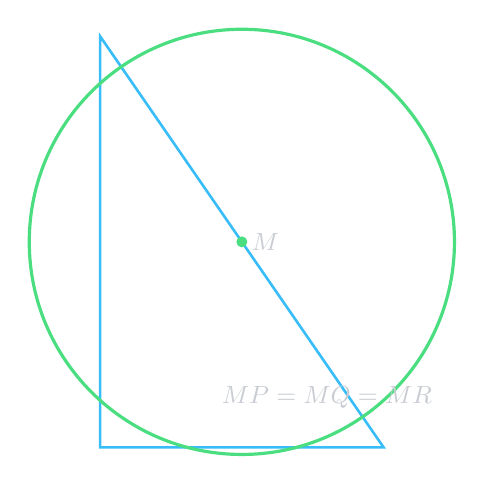
\begin{tikzpicture}[scale=0.9]
  \coordinate (Q) at (0,0);
  \coordinate (P) at (4,0);
  \coordinate (R) at (0,5.8);
  \coordinate (M) at ($(P)!0.5!(R)$);

  \draw[tri] (P)--(Q)--(R)--cycle;
  \draw[special] (M) circle[radius=3.0]; % circumcircle (schematic)
  \node[pt] at (M) {};
  \node[labm,right] at (M) {$M$};

  \node[labm] at ($(M)+(1.2,-2.2)$) {$MP=MQ=MR$};
\end{tikzpicture}
}
\end{QAPair}

% ============================================================
% Q3(c) - Perpendicular bisectors in obtuse triangle
\begin{QAPair}{Question 3 (c)}
\textcolor{gold}{\bfseries Question:} Show that perpendicular bisectors of $\triangle DEF$ are concurrent when $DE=5$ cm, $EF=4$ cm, $\angle E=120^\circ$.

\tcblower
\textcolor{green}{\bfseries Construction + circumcentre (step diagrams):}

\[
\begin{aligned}
\Step{1}\;& \text{At }E,\ \text{construct }120^\circ.\\
\Step{2}\;& \text{On arms, mark }ED=5\text{ cm and }EF=4\text{ cm.}\\
\Step{3}\;& \text{Join }DF\text{ to form }\triangle DEF.\\
\Step{4}\;& \text{Draw perpendicular bisector of }DE.\\
\Step{5}\;& \text{Draw perpendicular bisector of }EF;\ \text{they meet at }O.\\
\Step{6}\;& \text{Perp bisector of }DF\text{ also passes through }O \Rightarrow \text{concurrent at }O\ (\text{outside}).
\end{aligned}
\]

\StepPic{Step 1 (At $E$ construct $120^\circ$)}{
\begin{tikzpicture}[scale=1.0]
  \coordinate (E) at (0,0);
  \draw[aux] (E)--+(5.2,0);
  \draw[aux] (E)--+(120:5.2);
  \draw[aux] (E) ++(1.0,0) arc(0:120:1.0);
  \node[labm] at ($(E)+(0.35,1.1)$) {$120^\circ$};
  \node[pt] at (E) {};
  \node[labm,below] at (E) {$E$};
\end{tikzpicture}
}

\StepPic{Step 2 (Mark $ED=5$ and $EF=4$)}{
\begin{tikzpicture}[scale=1.0]
  \coordinate (E) at (0,0);
  \coordinate (F) at (4,0);
  \coordinate (D) at ($(E)+(120:5)$);

  \draw[tri] (E)--(F);
  \draw[tri] (E)--(D);

  \node[pt] at (E) {}; \node[pt] at (F) {}; \node[pt] at (D) {};
  \node[labm,below] at (E) {$E$};
  \node[labm,below right] at (F) {$F$};
  \node[labm,above left] at (D) {$D$};

  \node[labm,below] at ($(E)!0.5!(F)$) {$4$ cm};
  \node[labm,left] at ($(E)!0.5!(D)$) {$5$ cm};
\end{tikzpicture}
}

\StepPic{Step 3 (Join $DF$ to form triangle)}{
\begin{tikzpicture}[scale=1.0]
  \coordinate (E) at (0,0);
  \coordinate (F) at (4,0);
  \coordinate (D) at ($(E)+(120:5)$);

  \draw[tri] (D)--(E)--(F)--cycle;

  \node[pt] at (E) {}; \node[pt] at (F) {}; \node[pt] at (D) {};
  \node[labm,below] at (E) {$E$};
  \node[labm,below right] at (F) {$F$};
  \node[labm,above left] at (D) {$D$};

  \node[labm] at ($(E)+(0.35,1.1)$) {$120^\circ$};
\end{tikzpicture}
}

\StepPic{Step 4 (Draw perpendicular bisector of $DE$)}{
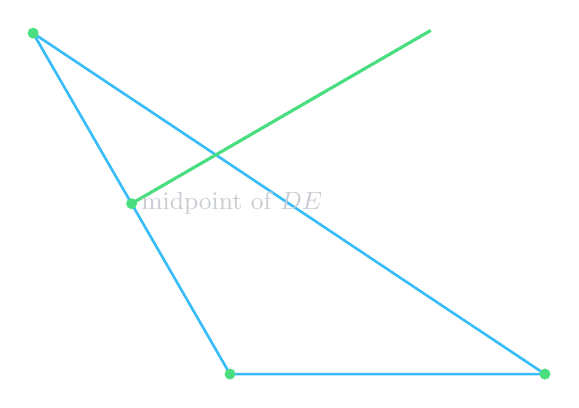
\begin{tikzpicture}[scale=1.0]
  \coordinate (E) at (0,0);
  \coordinate (F) at (4,0);
  \coordinate (D) at ($(E)+(120:5)$);
  \coordinate (Mde) at ($(D)!0.5!(E)$);

  \draw[tri] (D)--(E)--(F)--cycle;
  \draw[special] (Mde)--+(3.8,2.2); % schematic perpendicular bisector line
  \node[pt] at (Mde) {};
  \node[labm,right] at (Mde) {midpoint of $DE$};

  \node[pt] at (E) {}; \node[pt] at (F) {}; \node[pt] at (D) {};
\end{tikzpicture}
}

\StepPic{Step 5 (Draw perpendicular bisector of $EF$; intersection is $O$)}{
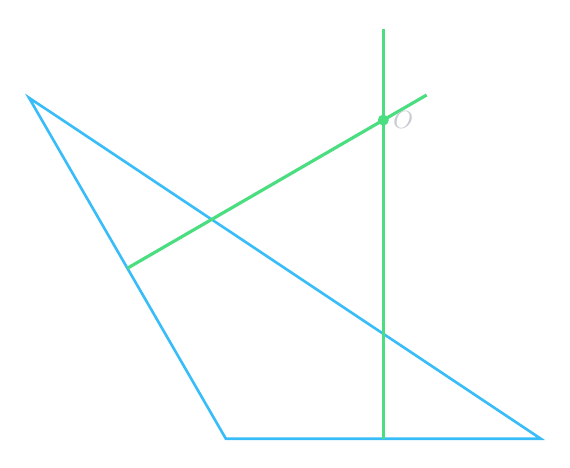
\begin{tikzpicture}[scale=1.0]
  \coordinate (E) at (0,0);
  \coordinate (F) at (4,0);
  \coordinate (D) at ($(E)+(120:5)$);

  \coordinate (Mde) at ($(D)!0.5!(E)$);
  \coordinate (Mef) at ($(E)!0.5!(F)$);

  \path[name path=bde] (Mde) -- +(3.8,2.2);
  \path[name path=bef] (Mef) -- +(0,5.2);
  \path[name intersections={of=bde and bef, by=O}];

  \draw[tri] (D)--(E)--(F)--cycle;
  \draw[special] (Mde)--+(3.8,2.2);
  \draw[special] (Mef)--+(0,5.2);

  \node[pt] at (O) {};
  \node[labm,right] at (O) {$O$};
\end{tikzpicture}
}

\StepPic{Step 6 (Third bisector also passes through $O$; $O$ is outside)}{
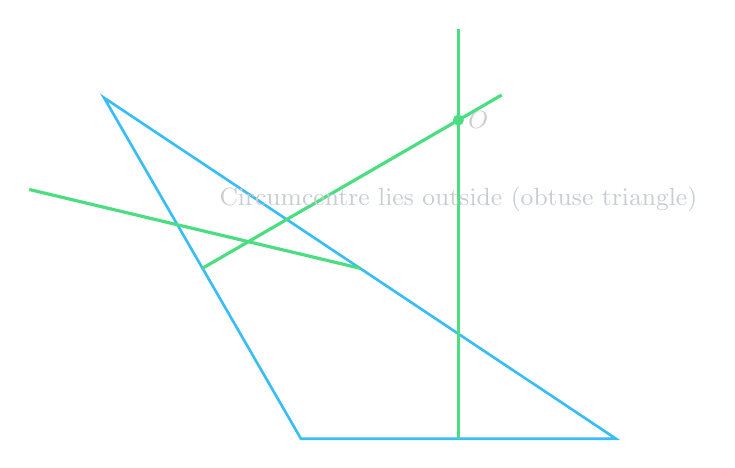
\begin{tikzpicture}[scale=1.0]
  \coordinate (E) at (0,0);
  \coordinate (F) at (4,0);
  \coordinate (D) at ($(E)+(120:5)$);

  \coordinate (Mde) at ($(D)!0.5!(E)$);
  \coordinate (Mef) at ($(E)!0.5!(F)$);
  \coordinate (Mdf) at ($(D)!0.5!(F)$);

  \path[name path=bde] (Mde) -- +(3.8,2.2);
  \path[name path=bef] (Mef) -- +(0,5.2);
  \path[name intersections={of=bde and bef, by=O}];

  \draw[tri] (D)--(E)--(F)--cycle;
  \draw[special] (Mde)--+(3.8,2.2);
  \draw[special] (Mef)--+(0,5.2);
  \draw[special] (Mdf)--+(-4.2,1.0);

  \node[pt] at (O) {};
  \node[labm,right] at (O) {$O$};
  \node[labm] at ($(O)+(0.0,-1.0)$) {Circumcentre lies outside (obtuse triangle)};
\end{tikzpicture}
}
\end{QAPair}

% ============================================================
% Q4(a) - Medians concurrent
\begin{QAPair}{Question 4 (a)}
\textcolor{gold}{\bfseries Question:} Show that medians of $\triangle ABC$ are concurrent when $AB=5.8$ cm, $BC=5$ cm, $\angle B=45^\circ$.

\tcblower
\textcolor{green}{\bfseries Construction + centroid (step diagrams):}

\[
\begin{aligned}
\Step{1}\;& \text{Draw }BC=5\text{ cm.}\\
\Step{2}\;& \text{At }B,\ \text{construct }45^\circ\text{ and draw ray }BA.\\
\Step{3}\;& \text{On ray }BA,\ \text{mark }AB=5.8\text{ cm to locate }A.\\
\Step{4}\;& \text{Join }A\text{ to }C \text{ to form }\triangle ABC.\\
\Step{5}\;& \text{Mark midpoints }D \text{ of }BC,\ E \text{ of }CA,\ F \text{ of }AB.\\
\Step{6}\;& \text{Draw medians }AD,\ BE,\ CF;\ \text{they meet at }G\ (\text{centroid}).
\end{aligned}
\]

\StepPic{Step 1 (Draw $BC=5$ cm)}{

\begin{tikzpicture}[scale=1.0]
  \coordinate (B) at (0,0);
  \coordinate (C) at (5,0);
  \draw[tri] (B)--(C);
  \node[pt] at (B) {}; \node[pt] at (C) {};
  \node[labm,below left] at (B) {$B$};
  \node[labm,below right] at (C) {$C$};
  \node[labm,below] at ($(B)!0.5!(C)$) {$5$ cm};
\end{tikzpicture}
}

\StepPic{Step 2 (At $B$, make $45^\circ$ ray $BA$)}{
\begin{tikzpicture}[scale=1.0]
  \coordinate (B) at (0,0);
  \coordinate (C) at (5,0);
  \draw[tri] (B)--(C);

  \draw[aux] (B)--+(45:6.0);
  \draw[aux] (B) ++(1.0,0) arc(0:45:1.0);
  \node[labm] at ($(B)+(0.95,0.35)$) {$45^\circ$};

  \node[pt] at (B) {}; \node[pt] at (C) {};
  \node[labm,below left] at (B) {$B$};
  \node[labm,below right] at (C) {$C$};
\end{tikzpicture}
}

\StepPic{Step 3 (Mark $AB=5.8$ cm to locate $A$)}{
\begin{tikzpicture}[scale=0.95]
  \coordinate (B) at (0,0);
  \coordinate (C) at (5,0);
  \coordinate (A) at ($(B)+(45:5.8)$);

  \draw[tri] (B)--(C);
  \draw[aux] (B)--+(45:6.2);

  \node[pt] at (A) {}; \node[pt] at (B) {}; \node[pt] at (C) {};
  \node[labm,above] at (A) {$A$};
  \node[labm,below left] at (B) {$B$};
  \node[labm,below right] at (C) {$C$};

  \node[labm] at ($(B)!0.55!(A)$) {$AB=5.8$ cm};
\end{tikzpicture}
}

\StepPic{Step 4 (Join $A$ to $C$ to form $\triangle ABC$)}{
\begin{tikzpicture}[scale=0.95]
  \coordinate (B) at (0,0);
  \coordinate (C) at (5,0);
  \coordinate (A) at ($(B)+(45:5.8)$);

  \draw[tri] (A)--(B)--(C)--cycle;

  \node[pt] at (A) {}; \node[pt] at (B) {}; \node[pt] at (C) {};
  \node[labm,above] at (A) {$A$};
  \node[labm,below left] at (B) {$B$};
  \node[labm,below right] at (C) {$C$};
\end{tikzpicture}
}

\StepPic{Step 5 (Mark midpoints $D,E,F$)}{
\begin{tikzpicture}[scale=0.95]
  \coordinate (B) at (0,0);
  \coordinate (C) at (5,0);
  \coordinate (A) at ($(B)+(45:5.8)$);

  \coordinate (D) at ($(B)!0.5!(C)$);
  \coordinate (E) at ($(C)!0.5!(A)$);
  \coordinate (F) at ($(A)!0.5!(B)$);

  \draw[tri] (A)--(B)--(C)--cycle;
  \node[pt] at (D) {}; \node[pt] at (E) {}; \node[pt] at (F) {};
  \node[labm,below] at (D) {$D$};
  \node[labm,right] at (E) {$E$};
  \node[labm,left] at (F) {$F$};

  \node[pt] at (A) {}; \node[pt] at (B) {}; \node[pt] at (C) {};
  \node[labm,above] at (A) {$A$};
  \node[labm,below left] at (B) {$B$};
  \node[labm,below right] at (C) {$C$};
\end{tikzpicture}
}

\StepPic{Step 6 (Draw medians; they meet at $G$)}{
\begin{tikzpicture}[scale=0.95]
  \coordinate (B) at (0,0);
  \coordinate (C) at (5,0);
  \coordinate (A) at ($(B)+(45:5.8)$);

  \coordinate (D) at ($(B)!0.5!(C)$);
  \coordinate (E) at ($(C)!0.5!(A)$);
  \coordinate (F) at ($(A)!0.5!(B)$);

  % centroid (barycentric equal weights)
  \coordinate (G) at (barycentric cs:A=1,B=1,C=1);

  \draw[tri] (A)--(B)--(C)--cycle;
  \draw[special] (A)--(D);
  \draw[special] (B)--(E);
  \draw[special] (C)--(F);

  \node[pt] at (G) {};
  \node[labm,right] at (G) {$G$};

  \node[pt] at (A) {}; \node[pt] at (B) {}; \node[pt] at (C) {};
  \node[labm,above] at (A) {$A$};
  \node[labm,below left] at (B) {$B$};
  \node[labm,below right] at (C) {$C$};

  \node[labm] at ($(G)+(0.0,-1.0)$) {All 3 medians meet at $G$};
\end{tikzpicture}
}
\end{QAPair}

% ============================================================
% Q4(b) - Medians concurrent (ASA triangle)
\begin{QAPair}{Question 4 (b)}
\textcolor{gold}{\bfseries Question:} Show that medians of $\triangle DEF$ are concurrent when $DE=6$ cm, $\angle D=90^\circ$, $\angle E=30^\circ$.

\tcblower
\textcolor{green}{\bfseries Construction + centroid (step diagrams):}

First, $\angle F = 180^\circ-(90^\circ+30^\circ)=60^\circ$.

\[
\begin{aligned}
\Step{1}\;& \text{Draw }DE=6\text{ cm.}\\
\Step{2}\;& \text{At }D,\ \text{construct }90^\circ;\ \text{at }E,\ \text{construct }30^\circ.\\
\Step{3}\;& \text{Rays meet at }F;\ \text{join to form }\triangle DEF.\\
\Step{4}\;& \text{Mark midpoints of }DE,\ EF,\ FD.\\
\Step{5}\;& \text{Draw two medians; they meet at }G.\\
\Step{6}\;& \text{Third median also passes through }G \Rightarrow \text{concurrent at }G.
\end{aligned}
\]

\StepPic{Step 1 (Draw $DE=6$ cm)}{
\begin{tikzpicture}[scale=1.0]
  \coordinate (D) at (0,0);
  \coordinate (E) at (6,0);
  \draw[tri] (D)--(E);
  \node[pt] at (D) {}; \node[pt] at (E) {};
  \node[labm,below left] at (D) {$D$};
  \node[labm,below right] at (E) {$E$};
  \node[labm,below] at ($(D)!0.5!(E)$) {$6$ cm};
\end{tikzpicture}
}

\StepPic{Step 2 (Make $\angle D=90^\circ$ and $\angle E=30^\circ$ rays)}{
\begin{tikzpicture}[scale=1.0]
  \coordinate (D) at (0,0);
  \coordinate (E) at (6,0);
  \draw[tri] (D)--(E);

  \draw[aux] (D)--+(0,4.0);
  \RightMarkAt{D}
  \draw[aux] (E)--+(150:4.6); % 30 with ED (left), direction 180-30=150
  \draw[aux] (E) ++(-1.0,0) arc(180:150:1.0);
  \node[labm] at ($(E)+(-0.8,0.45)$) {$30^\circ$};

  \node[pt] at (D) {}; \node[pt] at (E) {};
  \node[labm,below left] at (D) {$D$};
  \node[labm,below right] at (E) {$E$};
\end{tikzpicture}
}

\StepPic{Step 3 (Rays meet at $F$; form triangle)}{
\begin{tikzpicture}[scale=0.95]
  \coordinate (D) at (0,0);
  \coordinate (E) at (6,0);

  \path[name path=rayD] (D) -- +(90:6);
  \path[name path=rayE] (E) -- +(150:6);
  \path[name intersections={of=rayD and rayE, by=F}];

  \draw[tri] (D)--(E)--(F)--cycle;
  \RightMarkAt{D}

  \node[pt] at (D) {}; \node[pt] at (E) {}; \node[pt] at (F) {};
  \node[labm,below left] at (D) {$D$};
  \node[labm,below right] at (E) {$E$};
  \node[labm,above] at (F) {$F$};
\end{tikzpicture}
}

\StepPic{Step 4 (Mark midpoints)}{
\begin{tikzpicture}[scale=0.95]
  \coordinate (D) at (0,0);
  \coordinate (E) at (6,0);

  \path[name path=rayD] (D) -- +(90:6);
  \path[name path=rayE] (E) -- +(150:6);
  \path[name intersections={of=rayD and rayE, by=F}];

  \coordinate (Mde) at ($(D)!0.5!(E)$);
  \coordinate (Mef) at ($(E)!0.5!(F)$);
  \coordinate (Mfd) at ($(F)!0.5!(D)$);

  \draw[tri] (D)--(E)--(F)--cycle;
  \node[pt] at (Mde) {}; \node[pt] at (Mef) {}; \node[pt] at (Mfd) {};
  \node[labm,below] at (Mde) {$M_1$};
  \node[labm,right] at (Mef) {$M_2$};
  \node[labm,left] at (Mfd) {$M_3$};

  \node[pt] at (D) {}; \node[pt] at (E) {}; \node[pt] at (F) {};
  \node[labm,below left] at (D) {$D$};
  \node[labm,below right] at (E) {$E$};
  \node[labm,above] at (F) {$F$};
\end{tikzpicture}
}

\StepPic{Step 5 (Draw two medians; intersection is $G$)}{
\begin{tikzpicture}[scale=0.95]
  \coordinate (D) at (0,0);
  \coordinate (E) at (6,0);

  \path[name path=rayD] (D) -- +(90:6);
  \path[name path=rayE] (E) -- +(150:6);
  \path[name intersections={of=rayD and rayE, by=F}];

  \coordinate (Mde) at ($(D)!0.5!(E)$);
  \coordinate (Mef) at ($(E)!0.5!(F)$);
  \coordinate (Mfd) at ($(F)!0.5!(D)$);

  \coordinate (G) at (barycentric cs:D=1,E=1,F=1);

  \draw[tri] (D)--(E)--(F)--cycle;
  \draw[special] (F)--(Mde);
  \draw[special] (D)--(Mef);

  \node[pt] at (G) {}; \node[labm,right] at (G) {$G$};
\end{tikzpicture}
}

\StepPic{Step 6 (Third median also passes through $G$)}{
\begin{tikzpicture}[scale=0.95]
  \coordinate (D) at (0,0);
  \coordinate (E) at (6,0);

  \path[name path=rayD] (D) -- +(90:6);
  \path[name path=rayE] (E) -- +(150:6);
  \path[name intersections={of=rayD and rayE, by=F}];

  \coordinate (Mde) at ($(D)!0.5!(E)$);
  \coordinate (Mef) at ($(E)!0.5!(F)$);
  \coordinate (Mfd) at ($(F)!0.5!(D)$);

  \coordinate (G) at (barycentric cs:D=1,E=1,F=1);

  \draw[tri] (D)--(E)--(F)--cycle;
  \draw[special] (F)--(Mde);
  \draw[special] (D)--(Mef);
  \draw[special] (E)--(Mfd);

  \node[pt] at (G) {}; \node[labm,right] at (G) {$G$};
  \node[labm] at ($(G)+(0.0,-1.0)$) {All medians meet at $G$};
\end{tikzpicture}
}
\end{QAPair}

% ============================================================
% Q5(a) - Orthocentre in right triangle
\begin{QAPair}{Question 5 (a)}
\textcolor{gold}{\bfseries Question:} Construct a right triangle $ABC$ such that $\angle B=90^\circ$. Find its orthocentre; where does it lie?

\tcblower
\textcolor{green}{\bfseries Step-by-step:}

\[
\begin{aligned}
\Step{1}\;& \text{Construct right angle at }B.\\
\Step{2}\;& \text{Choose points }A \text{ and }C \text{ on the two perpendicular arms; join }AC.\\
\Step{3}\;& \text{Triangle }ABC\text{ is formed (right-angled at }B).\\
\Step{4}\;& \text{Altitude from }A\text{ to }BC \text{ is }AB\ (\text{since }AB\perp BC).\\
\Step{5}\;& \text{Altitude from }C\text{ to }AB \text{ is }CB.\\
\Step{6}\;& AB \text{ and }CB \text{ meet at }B \Rightarrow \text{orthocentre is }B.
\end{aligned}
\]

\StepPic{Step 1 (Right angle at $B$)}{
\begin{tikzpicture}[scale=1.0]
  \coordinate (B) at (0,0);
  \draw[aux] (B)--+(4.8,0);
  \draw[aux] (B)--+(0,3.6);
  \RightMarkAt{B}
  \node[pt] at (B) {};
  \node[labm,below left] at (B) {$B$};
\end{tikzpicture}
}

\StepPic{Step 2 (Pick $A$ and $C$ on the arms)}{
\begin{tikzpicture}[scale=1.0]
  \coordinate (B) at (0,0);
  \coordinate (C) at (4.2,0);
  \coordinate (A) at (0,3.0);

  \draw[aux] (B)--(C);
  \draw[aux] (B)--(A);
  \RightMarkAt{B}

  \node[pt] at (B) {}; \node[pt] at (A) {}; \node[pt] at (C) {};
  \node[labm,below left] at (B) {$B$};
  \node[labm,left] at (A) {$A$};
  \node[labm,below right] at (C) {$C$};
\end{tikzpicture}
}

\StepPic{Step 3 (Join $A$ to $C$ to form $\triangle ABC$)}{
\begin{tikzpicture}[scale=1.0]
  \coordinate (B) at (0,0);
  \coordinate (C) at (4.2,0);
  \coordinate (A) at (0,3.0);

  \draw[tri] (A)--(B)--(C)--cycle;
  \RightMarkAt{B}

  \node[pt] at (B) {}; \node[pt] at (A) {}; \node[pt] at (C) {};
  \node[labm,below left] at (B) {$B$};
  \node[labm,left] at (A) {$A$};
  \node[labm,below right] at (C) {$C$};
\end{tikzpicture}
}

\StepPic{Step 4 (Altitude from $A$ is $AB$)}{
\begin{tikzpicture}[scale=1.0]
  \coordinate (B) at (0,0);
  \coordinate (C) at (4.2,0);
  \coordinate (A) at (0,3.0);

  \draw[tri] (A)--(B)--(C)--cycle;
  \RightMarkAt{B}
  \draw[special] (A)--(B);

  \node[labm] at ($(A)!0.5!(B)+(-0.4,0)$) {Altitude from $A$};
\end{tikzpicture}
}

\StepPic{Step 5 (Altitude from $C$ is $CB$)}{
\begin{tikzpicture}[scale=1.0]
  \coordinate (B) at (0,0);
  \coordinate (C) at (4.2,0);
  \coordinate (A) at (0,3.0);

  \draw[tri] (A)--(B)--(C)--cycle;
  \RightMarkAt{B}
  \draw[special] (A)--(B);
  \draw[special] (C)--(B);

  \node[labm] at ($(C)!0.5!(B)+(0,-0.4)$) {Altitude from $C$};
\end{tikzpicture}
}

\StepPic{Step 6 (They meet at $B$: orthocentre)}{
\begin{tikzpicture}[scale=1.0]
  \coordinate (B) at (0,0);
  \coordinate (C) at (4.2,0);
  \coordinate (A) at (0,3.0);

  \draw[tri] (A)--(B)--(C)--cycle;
  \RightMarkAt{B}
  \draw[special] (A)--(B);
  \draw[special] (C)--(B);

  \node[pt] at (B) {};
  \node[labm,below left] at (B) {$B(=H)$};
  \node[labm] at ($(B)+(2.4,2.4)$) {Orthocentre at right-angle vertex};
\end{tikzpicture}
}
\end{QAPair}

% ============================================================
% Q5(b) - Circumcentre in right triangle
\begin{QAPair}{Question 5 (b)}
\textcolor{gold}{\bfseries Question:} In the same triangle, find circumcentre $M$. Is $M$ the midpoint of hypotenuse $AC$? Is $BM=CM$?

\tcblower
\textcolor{green}{\bfseries Step-by-step (right triangle fact):}

\[
\begin{aligned}
\Step{1}\;& \text{Draw the hypotenuse }AC.\\
\Step{2}\;& \text{Find midpoint }M \text{ of }AC.\\
\Step{3}\;& \text{Draw circle with centre }M \text{ passing through }A \text{ and }C.\\
\Step{4}\;& \text{This circle also passes through }B\ (\text{property of right triangles}).\\
\Step{5}\;& MA=MB=MC\ (\text{all are radii}).\\
\Step{6}\;& \Rightarrow M \text{ is circumcentre and midpoint of }AC,\ \text{and }BM=CM.
\end{aligned}
\]

\StepPic{Step 1 (Triangle $ABC$ with hypotenuse $AC$)}{
\begin{tikzpicture}[scale=1.0]
  \coordinate (B) at (0,0);
  \coordinate (C) at (4.2,0);
  \coordinate (A) at (0,3.0);

  \draw[tri] (A)--(B)--(C)--cycle;
  \RightMarkAt{B}
  \draw[aux] (A)--(C);

  \node[pt] at (A) {}; \node[pt] at (B) {}; \node[pt] at (C) {};
  \node[labm,left] at (A) {$A$};
  \node[labm,below left] at (B) {$B$};
  \node[labm,below right] at (C) {$C$};
  \node[labm] at ($(A)!0.5!(C)+(0.6,0.0)$) {hypotenuse};
\end{tikzpicture}
}

\StepPic{Step 2 (Midpoint $M$ of $AC$)}{
\begin{tikzpicture}[scale=1.0]
  \coordinate (B) at (0,0);
  \coordinate (C) at (4.2,0);
  \coordinate (A) at (0,3.0);
  \coordinate (M) at ($(A)!0.5!(C)$);

  \draw[tri] (A)--(B)--(C)--cycle;
  \RightMarkAt{B}
  \draw[aux] (A)--(C);
  \node[pt] at (M) {};
  \node[labm,right] at (M) {$M$};
  \node[labm] at ($(M)+(0.0,-0.8)$) {midpoint of $AC$};
\end{tikzpicture}
}

\StepPic{Step 3 (Circle with centre $M$ through $A$ and $C$)}{
\begin{tikzpicture}[scale=1.0]
  \coordinate (B) at (0,0);
  \coordinate (C) at (4.2,0);
  \coordinate (A) at (0,3.0);
  \coordinate (M) at ($(A)!0.5!(C)$);

  \draw[tri] (A)--(B)--(C)--cycle;
  \RightMarkAt{B}
  \draw[special] (M) circle[radius=2.5]; % schematic
  \node[pt] at (M) {};
  \node[labm,right] at (M) {$M$};
\end{tikzpicture}
}

\StepPic{Step 4 (Check: $B$ lies on the circle)}{
\begin{tikzpicture}[scale=1.0]
  \coordinate (B) at (0,0);
  \coordinate (C) at (4.2,0);
  \coordinate (A) at (0,3.0);
  \coordinate (M) at ($(A)!0.5!(C)$);

  \draw[tri] (A)--(B)--(C)--cycle;
  \RightMarkAt{B}
  \draw[special] (M) circle[radius=2.5];
  \draw[aux] (M)--(B);
  \node[labm] at ($(M)!0.5!(B)+(0.2,0.2)$) {$MB$};
\end{tikzpicture}
}

\StepPic{Step 5 (All radii equal: $MA=MB=MC$)}{
\begin{tikzpicture}[scale=1.0]
  \coordinate (B) at (0,0);
  \coordinate (C) at (4.2,0);
  \coordinate (A) at (0,3.0);
  \coordinate (M) at ($(A)!0.5!(C)$);

  \draw[tri] (A)--(B)--(C)--cycle;
  \draw[special] (M) circle[radius=2.5];
  \draw[aux] (M)--(A);
  \draw[aux] (M)--(B);
  \draw[aux] (M)--(C);

  \node[pt] at (M) {};
  \node[labm,right] at (M) {$M$};
  \node[labm] at ($(M)+(1.1,-2.2)$) {$MA=MB=MC$};
\end{tikzpicture}
}

\StepPic{Step 6 (Conclusion)}{
\begin{tikzpicture}[scale=1.0]
  \coordinate (B) at (0,0);
  \coordinate (C) at (4.2,0);
  \coordinate (A) at (0,3.0);
  \coordinate (M) at ($(A)!0.5!(C)$);

  \draw[tri] (A)--(B)--(C)--cycle;
  \draw[special] (M) circle[radius=2.5];
  \node[pt] at (M) {};
  \node[labm,right] at (M) {$M$};
  \node[labm] at ($(M)+(0.0,-2.8)$) {Circumcentre = midpoint of hypotenuse};
\end{tikzpicture}
}
\end{QAPair}

% ============================================================
% Q6 - Obtuse triangle: circumcentre and orthocentre outside
\begin{QAPair}{Question 6}
\textcolor{gold}{\bfseries Question:} Construct an obtuse-angled triangle $DEF$. Find its (a) circumcentre (b) orthocentre. Check whether they lie inside or outside the triangle.

\tcblower
\textcolor{green}{\bfseries Step-by-step:}

\[
\begin{aligned}
\Step{1}\;& \text{Draw any obtuse triangle }DEF\ (\text{one angle } > 90^\circ).\\
\Step{2}\;& \text{Circumcentre }O:\ \text{draw perpendicular bisectors of two sides; they meet at }O.\\
\Step{3}\;& \text{Orthocentre }H:\ \text{draw two altitudes; they meet at }H.\\
\Step{4}\;& \text{In an obtuse triangle, perpendicular bisectors meet outside } \Rightarrow O \text{ is outside.}\\
\Step{5}\;& \text{Also, altitudes intersect outside } \Rightarrow H \text{ is outside.}\\
\Step{6}\;& \text{Mark and confirm both lie outside the triangle.}
\end{aligned}
\]

\StepPic{Step 1 (Choose an obtuse triangle)}{
\begin{tikzpicture}[scale=1.0]
  \coordinate (E) at (0,0);
  \coordinate (F) at (5.2,0.6);
  \coordinate (D) at (-1.4,2.8);

  \draw[tri] (D)--(E)--(F)--cycle;

  \node[pt] at (D) {}; \node[pt] at (E) {}; \node[pt] at (F) {};
  \node[labm,above] at (D) {$D$};
  \node[labm,below] at (E) {$E$};
  \node[labm,right] at (F) {$F$};

  \node[labm] at ($(E)+(0.8,1.2)$) {one angle $>90^\circ$};
\end{tikzpicture}
}

\StepPic{Step 2 (Perpendicular bisectors meet at $O$ outside)}{
\begin{tikzpicture}[scale=1.0]
  \coordinate (E) at (0,0);
  \coordinate (F) at (5.2,0.6);
  \coordinate (D) at (-1.4,2.8);

  \coordinate (Mde) at ($(D)!0.5!(E)$);
  \coordinate (Mef) at ($(E)!0.5!(F)$);

  \path[name path=bde] (Mde)--+(4.5,2.0);
  \path[name path=bef] (Mef)--+(0,5.0);
  \path[name intersections={of=bde and bef, by=O}];

  \draw[tri] (D)--(E)--(F)--cycle;
  \draw[special] (Mde)--+(4.5,2.0);
  \draw[special] (Mef)--+(0,5.0);

  \node[pt] at (O) {}; \node[labm,right] at (O) {$O$};
  \node[labm] at ($(O)+(0.2,-0.8)$) {circumcentre (outside)};
\end{tikzpicture}
}

\StepPic{Step 3 (Altitudes meet at $H$ outside)}{
\begin{tikzpicture}[scale=1.0]
  \coordinate (E) at (0,0);
  \coordinate (F) at (5.2,0.6);
  \coordinate (D) at (-1.4,2.8);

  \coordinate (A1) at ($(E)!(D)!(F)$); % foot from D to EF (schematic)
  \coordinate (A2) at ($(D)!(F)!(E)$); % foot from F to DE (schematic)

  \path[name path=altD] (D)--(A1);
  \path[name path=altF] (F)--(A2);
  \path[name intersections={of=altD and altF, by=H}];

  \draw[tri] (D)--(E)--(F)--cycle;
  \draw[special] (D)--(A1);
  \draw[special] (F)--(A2);

  \node[pt] at (H) {}; \node[labm,right] at (H) {$H$};
  \node[labm] at ($(H)+(0.2,-0.8)$) {orthocentre (outside)};
\end{tikzpicture}
}

\StepPic{Step 4 (Show both points are outside)}{
\begin{tikzpicture}[scale=1.0]
  \coordinate (E) at (0,0);
  \coordinate (F) at (5.2,0.6);
  \coordinate (D) at (-1.4,2.8);

  % circumcentre (schematic)
  \coordinate (Mde) at ($(D)!0.5!(E)$);
  \coordinate (Mef) at ($(E)!0.5!(F)$);
  \path[name path=bde] (Mde)--+(4.5,2.0);
  \path[name path=bef] (Mef)--+(0,5.0);
  \path[name intersections={of=bde and bef, by=O}];

  % orthocentre (schematic)
  \coordinate (A1) at ($(E)!(D)!(F)$);
  \coordinate (A2) at ($(D)!(F)!(E)$);
  \path[name path=altD] (D)--(A1);
  \path[name path=altF] (F)--(A2);
  \path[name intersections={of=altD and altF, by=H}];

  \draw[tri] (D)--(E)--(F)--cycle;
  \draw[special] (Mde)--+(4.5,2.0);
  \draw[special] (Mef)--+(0,5.0);
  \draw[special] (D)--(A1);
  \draw[special] (F)--(A2);

  \node[pt] at (O) {}; \node[labm,right] at (O) {$O$};
  \node[pt] at (H) {}; \node[labm,right] at (H) {$H$};

  \node[labm] at ($(E)+(1.2,-1.0)$) {$O$ and $H$ are outside for obtuse triangles};
\end{tikzpicture}
}
\end{QAPair}

% ============================================================
% Q7 - Isosceles: centroid and incentre
\begin{QAPair}{Question 7}
\textcolor{gold}{\bfseries Question:} Construct an isosceles triangle and find its (a) centroid (b) incentre.

\tcblower
\textcolor{green}{\bfseries Step-by-step (with diagrams):}

\textcolor{cyan}{\bfseries (a) Centroid $G$}
\[
\begin{aligned}
\Step{1}\;& \text{Draw base }BC.\\
\Step{2}\;& \text{Construct perpendicular bisector of }BC\text{ and choose }A \text{ on it so that }AB=AC.\\
\Step{3}\;& \text{Join }AB\text{ and }AC\text{ to make isosceles }\triangle ABC.\\
\Step{4}\;& \text{Mark midpoints of the sides.}\\
\Step{5}\;& \text{Draw two medians; they meet at }G.\\
\Step{6}\;& \text{Third median also passes through }G.
\end{aligned}
\]

\StepPic{(a) Step 1 (Draw base $BC$)}{
\begin{tikzpicture}[scale=1.0]
  \coordinate (B) at (0,0);
  \coordinate (C) at (5.2,0);
  \draw[tri] (B)--(C);
  \node[pt] at (B) {}; \node[pt] at (C) {};
  \node[labm,below left] at (B) {$B$};
  \node[labm,below right] at (C) {$C$};
\end{tikzpicture}
}

\StepPic{(a) Step 2 (Perpendicular bisector of $BC$; choose $A$ on it)}{
\begin{tikzpicture}[scale=1.0]
  \coordinate (B) at (0,0);
  \coordinate (C) at (5.2,0);
  \coordinate (M) at ($(B)!0.5!(C)$);
  \coordinate (A) at ($(M)+(0,3.2)$);

  \draw[tri] (B)--(C);
  \draw[aux] (M)--+(0,4.0);

  \node[pt] at (A) {}; \node[pt] at (B) {}; \node[pt] at (C) {};
  \node[labm,above] at (A) {$A$};
  \node[labm,below left] at (B) {$B$};
  \node[labm,below right] at (C) {$C$};

  \node[labm] at ($(M)+(0.9,1.8)$) {perp bisector of $BC$};
\end{tikzpicture}
}

\StepPic{(a) Step 3 (Join to form isosceles triangle $AB=AC$)}{
\begin{tikzpicture}[scale=1.0]
  \coordinate (B) at (0,0);
  \coordinate (C) at (5.2,0);
  \coordinate (A) at (2.6,3.2);

  \draw[tri] (A)--(B)--(C)--cycle;
  \node[pt] at (A) {}; \node[pt] at (B) {}; \node[pt] at (C) {};
  \node[labm,above] at (A) {$A$};
  \node[labm,below left] at (B) {$B$};
  \node[labm,below right] at (C) {$C$};
  \node[labm] at ($(A)+(0,0.45)$) {$AB=AC$};
\end{tikzpicture}
}

\StepPic{(a) Step 4 (Mark midpoints)}{
\begin{tikzpicture}[scale=1.0]
  \coordinate (B) at (0,0);
  \coordinate (C) at (5.2,0);
  \coordinate (A) at (2.6,3.2);

  \coordinate (D) at ($(B)!0.5!(C)$);
  \coordinate (E) at ($(C)!0.5!(A)$);
  \coordinate (F) at ($(A)!0.5!(B)$);

  \draw[tri] (A)--(B)--(C)--cycle;
  \node[pt] at (D) {}; \node[pt] at (E) {}; \node[pt] at (F) {};
  \node[labm,below] at (D) {$D$};
  \node[labm,right] at (E) {$E$};
  \node[labm,left] at (F) {$F$};
\end{tikzpicture}
}

\StepPic{(a) Step 5 (Draw two medians; meet at $G$)}{
\begin{tikzpicture}[scale=1.0]
  \coordinate (B) at (0,0);
  \coordinate (C) at (5.2,0);
  \coordinate (A) at (2.6,3.2);
  \coordinate (D) at ($(B)!0.5!(C)$);
  \coordinate (E) at ($(C)!0.5!(A)$);
  \coordinate (F) at ($(A)!0.5!(B)$);
  \coordinate (G) at (barycentric cs:A=1,B=1,C=1);

  \draw[tri] (A)--(B)--(C)--cycle;
  \draw[special] (A)--(D);
  \draw[special] (B)--(E);
  \node[pt] at (G) {}; \node[labm,right] at (G) {$G$};
\end{tikzpicture}
}

\StepPic{(a) Step 6 (Third median also passes through $G$)}{
\begin{tikzpicture}[scale=1.0]
  \coordinate (B) at (0,0);
  \coordinate (C) at (5.2,0);
  \coordinate (A) at (2.6,3.2);
  \coordinate (D) at ($(B)!0.5!(C)$);
  \coordinate (E) at ($(C)!0.5!(A)$);
  \coordinate (F) at ($(A)!0.5!(B)$);
  \coordinate (G) at (barycentric cs:A=1,B=1,C=1);

  \draw[tri] (A)--(B)--(C)--cycle;
  \draw[special] (A)--(D);
  \draw[special] (B)--(E);
  \draw[special] (C)--(F);
  \node[pt] at (G) {}; \node[labm,right] at (G) {$G$};
\end{tikzpicture}
}

\textcolor{cyan}{\bfseries (b) Incentre $I$}
\[
\begin{aligned}
\Step{1}\;& \text{Take the same isosceles triangle }ABC.\\
\Step{2}\;& \text{Draw bisector of }\angle A.\\
\Step{3}\;& \text{Draw bisector of }\angle B.\\
\Step{4}\;& \text{They meet at }I.\\
\Step{5}\;& \text{Draw bisector of }\angle C.\\
\Step{6}\;& \text{It also passes through }I \Rightarrow I \text{ is incentre.}
\end{aligned}
\]

\StepPic{(b) Step 1 (Triangle $ABC$)}{
\begin{tikzpicture}[scale=1.0]
  \coordinate (B) at (0,0);
  \coordinate (C) at (5.2,0);
  \coordinate (A) at (2.6,3.2);
  \draw[tri] (A)--(B)--(C)--cycle;
\end{tikzpicture}
}

\StepPic{(b) Step 2 (Draw bisector of $\angle A$)}{
\begin{tikzpicture}[scale=1.0]
  \coordinate (B) at (0,0);
  \coordinate (C) at (5.2,0);
  \coordinate (A) at (2.6,3.2);
  \coordinate (I) at (2.6,1.2); % schematic
  \draw[tri] (A)--(B)--(C)--cycle;
  \draw[special] (A)--(I);
  \node[pt] at (I) {};
\end{tikzpicture}
}

\StepPic{(b) Step 3 (Draw bisector of $\angle B$)}{
\begin{tikzpicture}[scale=1.0]
  \coordinate (B) at (0,0);
  \coordinate (C) at (5.2,0);
  \coordinate (A) at (2.6,3.2);
  \coordinate (I) at (2.6,1.2);
  \draw[tri] (A)--(B)--(C)--cycle;
  \draw[special] (A)--(I);
  \draw[special] (B)--(I);
  \node[pt] at (I) {};
\end{tikzpicture}
}

\StepPic{(b) Step 4 (Intersection is $I$)}{
\begin{tikzpicture}[scale=1.0]
  \coordinate (B) at (0,0);
  \coordinate (C) at (5.2,0);
  \coordinate (A) at (2.6,3.2);
  \coordinate (I) at (2.6,1.2);
  \draw[tri] (A)--(B)--(C)--cycle;
  \draw[special] (A)--(I);
  \draw[special] (B)--(I);
  \node[pt] at (I) {};
  \node[labm,right] at (I) {$I$};
\end{tikzpicture}
}

\StepPic{(b) Step 5 (Draw bisector of $\angle C$)}{
\begin{tikzpicture}[scale=1.0]
  \coordinate (B) at (0,0);
  \coordinate (C) at (5.2,0);
  \coordinate (A) at (2.6,3.2);
  \coordinate (I) at (2.6,1.2);
  \draw[tri] (A)--(B)--(C)--cycle;
  \draw[special] (A)--(I);
  \draw[special] (B)--(I);
  \draw[special] (C)--(I);
  \node[pt] at (I) {};
\end{tikzpicture}
}

\StepPic{(b) Step 6 (All bisectors meet at $I$: incentre)}{
\begin{tikzpicture}[scale=1.0]
  \coordinate (B) at (0,0);
  \coordinate (C) at (5.2,0);
  \coordinate (A) at (2.6,3.2);
  \coordinate (I) at (2.6,1.2);
  \draw[tri] (A)--(B)--(C)--cycle;
  \draw[special] (A)--(I);
  \draw[special] (B)--(I);
  \draw[special] (C)--(I);
  \node[pt] at (I) {};
  \node[labm,right] at (I) {$I$};
  \node[labm] at ($(I)+(0.0,-1.0)$) {Incentre (concurrency point)};
\end{tikzpicture}
}
\end{QAPair}

% ============================================================
% Q8 - Identification (still shown step-by-step highlighting)
\begin{QAPair}{Question 8}
\textcolor{gold}{\bfseries Question:} Recognize altitudes, perpendicular bisectors and medians in the given figures (a) and (b).

\tcblower
\textcolor{green}{\bfseries Step-by-step highlighting:}

\textcolor{cyan}{\bfseries Figure (a)}
\[
\begin{aligned}
\Step{1}\;& \text{Draw the given triangle with points and the given segments.}\\
\Step{2}\;& \text{Highlight the segment where a midpoint is shown }(BD=DC)\Rightarrow AD\text{ is a median.}\\
\Step{3}\;& \text{Highlight the segment with a right-angle mark to a side }\Rightarrow \text{an altitude.}\\
\Step{4}\;& \text{Highlight the line through a midpoint and perpendicular to a side }\Rightarrow \text{a perpendicular bisector.}
\end{aligned}
\]

\StepPic{(a) Step 1 (Given figure)}{
\begin{tikzpicture}[scale=0.95]
  \coordinate (B) at (0,0);
  \coordinate (C) at (4.2,0);
  \coordinate (A) at (0.8,3.0);
  \coordinate (D) at ($(B)!0.5!(C)$);
  \coordinate (E) at ($(A)!0.55!(C)$);
  \coordinate (M) at ($(A)!0.5!(B)$);

  \draw[tri] (A)--(B)--(C)--cycle;
  \draw[aux] (A)--(D);
  \draw[aux] (B)--(E);

  % right angle mark at E (schematic)
  \draw[aux] (E) -- ++(-0.25,0.12) -- ++(0.12,0.25);

  % tick marks BD=DC
  \draw[aux] ($(B)!0.5!(D)$) ++(0,0.12) -- ++(0,-0.24);
  \draw[aux] ($(D)!0.5!(C)$) ++(0,0.12) -- ++(0,-0.24);

  \node[pt] at (A) {}; \node[pt] at (B) {}; \node[pt] at (C) {};
  \node[pt] at (D) {}; \node[pt] at (E) {};
  \node[labm,above] at (A) {$A$};
  \node[labm,below left] at (B) {$B$};
  \node[labm,below right] at (C) {$C$};
  \node[labm,below] at (D) {$D$};
  \node[labm,right] at (E) {$E$};
\end{tikzpicture}
}

\StepPic{(a) Step 2 (Median: highlight $AD$ since $D$ is midpoint of $BC$)}{
\begin{tikzpicture}[scale=0.95]
  \coordinate (B) at (0,0);
  \coordinate (C) at (4.2,0);
  \coordinate (A) at (0.8,3.0);
  \coordinate (D) at ($(B)!0.5!(C)$);

  \draw[tri] (A)--(B)--(C)--cycle;
  \draw[special] (A)--(D);

  % tick marks BD=DC
  \draw[aux] ($(B)!0.5!(D)$) ++(0,0.12) -- ++(0,-0.24);
  \draw[aux] ($(D)!0.5!(C)$) ++(0,0.12) -- ++(0,-0.24);

  \node[labm] at ($(A)!0.5!(D)+(0.6,0.0)$) {Median};
\end{tikzpicture}
}

\StepPic{(a) Step 3 (Altitude: highlight the perpendicular segment)}{
\begin{tikzpicture}[scale=0.95]
  \coordinate (B) at (0,0);
  \coordinate (C) at (4.2,0);
  \coordinate (A) at (0.8,3.0);
  \coordinate (E) at ($(A)!0.55!(C)$);

  \draw[tri] (A)--(B)--(C)--cycle;
  \draw[special] (B)--(E);

  \draw[aux] (E) -- ++(-0.25,0.12) -- ++(0.12,0.25);
  \node[labm] at ($(B)!0.5!(E)+(-0.2,0.2)$) {Altitude};
\end{tikzpicture}
}

\StepPic{(a) Step 4 (Perpendicular bisector: line through midpoint $\perp$ side)}{
\begin{tikzpicture}[scale=0.95]
  \coordinate (B) at (0,0);
  \coordinate (C) at (4.2,0);
  \coordinate (A) at (0.8,3.0);
  \coordinate (M) at ($(A)!0.5!(B)$);

  \draw[tri] (A)--(B)--(C)--cycle;

  % schematic perpendicular bisector through M
  \draw[special] (M)--+(2.8,0.0);
  \node[pt] at (M) {};
  \node[labm] at ($(M)+(1.1,0.35)$) {Perp bisector (shown)};
\end{tikzpicture}
}

\textcolor{cyan}{\bfseries Figure (b)}
\[
\begin{aligned}
\Step{1}\;& \text{Identify the right triangle (right angle at }S).\\
\Step{2}\;& \text{In a right triangle, midpoint of hypotenuse is circumcentre.}\\
\Step{3}\;& \text{Segments shown through midpoints and perpendicular to legs are perpendicular bisectors.}\\
\Step{4}\;& \text{Segment from right-angle vertex to midpoint of hypotenuse is a median.}
\end{aligned}
\]

\StepPic{(b) Step 1 (Given right triangle)}{
\begin{tikzpicture}[scale=0.95]
  \coordinate (P) at (0,0);
  \coordinate (S) at (4.2,0);
  \coordinate (R) at (4.2,3.0);

  \draw[tri] (P)--(S)--(R)--cycle;
  \draw[aux] (S) -- ++(-0.6,0) -- ++(0,0.6) -- ++(0.6,0);

  \node[pt] at (P) {}; \node[pt] at (S) {}; \node[pt] at (R) {};
  \node[labm,below left] at (P) {$P$};
  \node[labm,below] at (S) {$S$};
  \node[labm,right] at (R) {$R$};
\end{tikzpicture}
}

\StepPic{(b) Step 2 (Midpoint $U$ of hypotenuse $PR$)}{
\begin{tikzpicture}[scale=0.95]
  \coordinate (P) at (0,0);
  \coordinate (S) at (4.2,0);
  \coordinate (R) at (4.2,3.0);
  \coordinate (U) at ($(P)!0.5!(R)$);

  \draw[tri] (P)--(S)--(R)--cycle;
  \draw[aux] (P)--(R);
  \node[pt] at (U) {}; \node[labm,left] at (U) {$U$};
  \node[labm] at ($(U)+(1.0,-0.6)$) {midpoint of hypotenuse};
\end{tikzpicture}
}

\StepPic{(b) Step 3 (Perpendicular bisectors through midpoints)}{
\begin{tikzpicture}[scale=0.95]
  \coordinate (P) at (0,0);
  \coordinate (S) at (4.2,0);
  \coordinate (R) at (4.2,3.0);

  \coordinate (Q) at ($(P)!0.5!(S)$);
  \coordinate (T) at ($(S)!0.5!(R)$);
  \coordinate (U) at ($(P)!0.5!(R)$);

  \draw[tri] (P)--(S)--(R)--cycle;

  \draw[special] (U)--(Q);
  \draw[special] (U)--(T);

  \node[pt] at (Q) {}; \node[pt] at (T) {}; \node[pt] at (U) {};
  \node[labm,below] at (Q) {$Q$};
  \node[labm,right] at (T) {$T$};
  \node[labm,left] at (U) {$U$};

  \node[labm] at ($(U)+(1.3,1.0)$) {Perp bisectors};
\end{tikzpicture}
}

\StepPic{(b) Step 4 (Median from $S$ to midpoint $U$ of hypotenuse)}{
\begin{tikzpicture}[scale=0.95]
  \coordinate (P) at (0,0);
  \coordinate (S) at (4.2,0);
  \coordinate (R) at (4.2,3.0);
  \coordinate (U) at ($(P)!0.5!(R)$);

  \draw[tri] (P)--(S)--(R)--cycle;
  \draw[special] (S)--(U);

  \node[pt] at (U) {}; \node[labm,left] at (U) {$U$};
  \node[labm] at ($(S)!0.5!(U)+(-0.2,0.2)$) {Median};
\end{tikzpicture}
}
\end{QAPair}

\end{document}
